\chapter{Control}

\section{Adjusting a desired operating point}

\subsection{Terminology}


Consider the problem of setting a desired $Q_d$ flow rate at the pipeline system with head-discharge problem of $H_s$. If we simply connect a pump to the system, the provided flow rate will not be the desired one but the the flow rate corresponding to the intersection of the pump and pipeline curve. By controlling either the pump or the system (via valves), we can achieve the desired flow rate. However, it is typical that either the $Q_p$ flow rate of the pump or the $H_p$ head of the pump is not the same as that of the pipeline system

When making decisions on pump or fan control, we use two following important quantities.

\begin{description}
\item[Control efficiency.] This quantity is the ratio of the useful power and the input power, that is
\begin{equation}
\eta=\frac{P_{useful}}{P_{input}}=\frac{Q_d \rho g H_s(Q_d)}{Q_p \rho g H_p(Q_p)}
\end{equation}
%
\item[Specific energy consumption.] This quantity is the ratio of the input power and the flow rate, that is
\begin{equation}
\text{SEC}=\frac{P_{input}}{Q_d}=\frac{P_{input}}{V/t}=\frac{\text{energy consumed}}{\text{volume of fluid}},
\end{equation}
that is, the energy consumption of conveying 1 $m^3$ of fluid in the system.
\end{description}

We shall analyse three ways of control:

\begin{enumerate}
\item Control via a valve connected in series.
\item Control via a valve connected in parallel, i.e. by-pass valve.
\item Control via a changing the pump revolution number.
\end{enumerate}

\clearpage

\subsection{Valve in series}


%\begin{figure}
\begin{wrapfigure}{r}{0.6\textwidth}
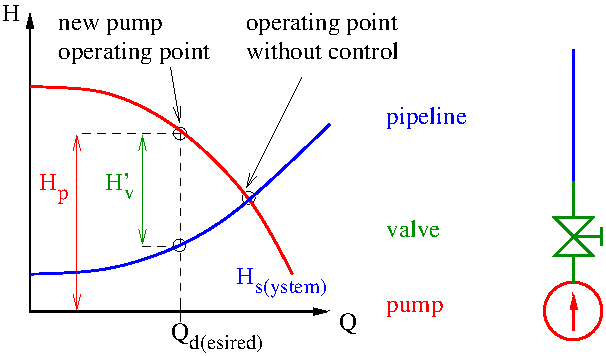
\includegraphics[width=0.6\textwidth]{figs/series_connection.pdf}
\caption{Control via a valve connected in series.}
\end{wrapfigure}
%\end{figure}

In the case of series valve control, we add a throttle valve at the pressure side of the pump. (And never at the suction side, due to the danger of cavitation!) As the three element are now connected in series, the flow rate is common, while the pressure will change. 

The efficiency is $\eta=\frac{Q_d \rho g H_s}{P_{pump}}$, where $P_{pump}=H_p\rho g Q_d/\eta_{pump}(Q_d)$, hence we have $\eta=\eta_{pump}(Q_d)H_s/H_p$. That is, the ratio of the system head and the pump head, multiplied by the efficiency of the pump at the operating point. The specific energy consumption is SEC$=\rho g H_p(Q_d)\eta_{pump}(Q_d)$. 

This type of control introduces new head loss at the pressure side, resulting in a higher overall pipeline loss, which than reduces the head of the pump. The power lost on the throttle valve is $P'_v=Q_d \rho g H'_v$.

\subsection{Bypass valve (parallel)}


%\begin{figure}
\begin{wrapfigure}{r}{0.6\textwidth}
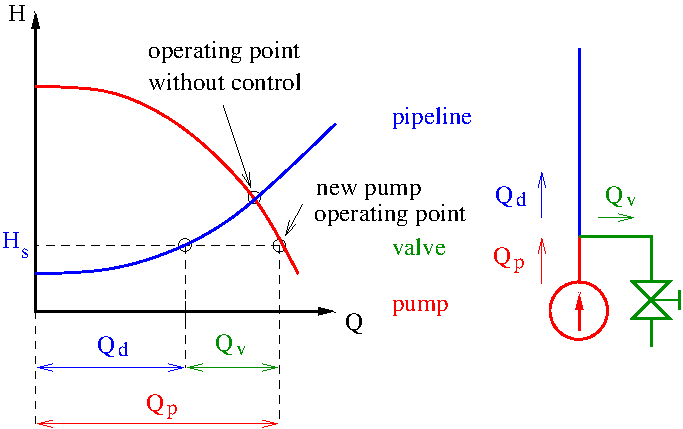
\includegraphics[width=0.6\textwidth]{figs/parallel_connection.pdf}
\caption{Control via a valve connected in series.}
\end{wrapfigure}
%\end{figure}

In the case of a bypass valve, we add a throttle valve parallel with the pump to allow backflow of unnecessary fluid into the suction-side reservoir.  As the three element are now connected in parallel, the flow rate adds up, while the pressure difference is the same. 

The efficiency is $\eta=\frac{Q_d \rho g H_s}{P_{pump}}$, where $P_{pump}=H_s\rho g Q_p/\eta_{pump}(Q_p)$, hence we have $\eta=\eta_{pump}(Q_p)Q_s/Q_p$. That is, the ratio of the desired flow rate and the pump flow rate, multiplied by the efficiency of the pump at the pump operating point. The specific energy consumption is SEC$=\rho g H_p(Q_p)\eta_{pump}(Q_p)$.

This type of control does not introduce new head loss, but allows a portion of the (too large) pump flow rate back to the reservoir. The power lost on the throttle valve is $P'_v=Q_v \rho g H_s$.

\section{Pump revolution number control}

A common way of setting pump flow rate is to vary the revolution number. Intuitively, decreasing the pump revolution number will result in lower flow rate, while increasing it will result in higher flow rate.

Combining the affinity laws $Q_2/Q_1=n_2/n_1$ and $H_2/H_1=n_2^2/n_1^2$ give $H_2=\left( H_1/Q_1^2\right)Q_2^2:=a\,Q_2^2$. This simply means that while changing the revolution number, the operating point moves along an \emph{central parabola} $a Q^2$ that starts from the origin and passes through the original point $\left( Q_1,H_1\right)$. \emph{The affinity law can be used only between point lying on the same central parabola.}

See the first problem in the next section for a worked example.

\subsection{Problems}

\noindent {\bf Problem \thesection.\theprob}\stepcounter{prob}

A pump running at $1470 [rpm]$ with $H_{pump}=45-2781 Q^2$ head delivers water into a pipeline with $H_{pipe}=20+1125Q^2$. Calculate the required revolution number for the reduced flow rate $Q'=0.05 [m^3/s]$. 

\vspace{0.5cm}
\begin{tabular}{cc}
    \begin{minipage}{9cm}
	\begin{center}
	    \resizebox{9cm}{!}{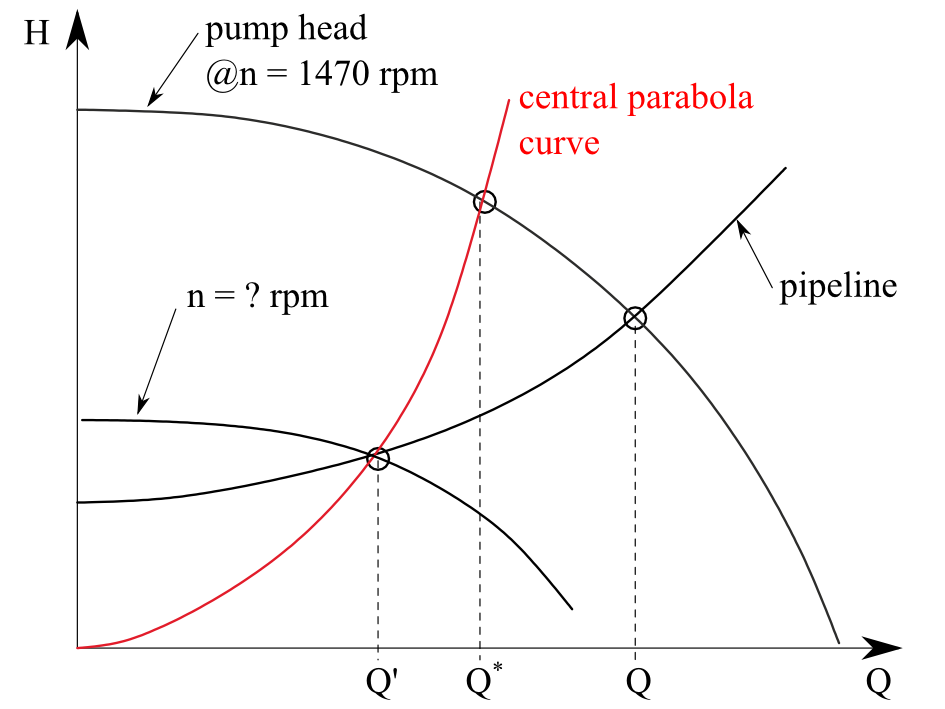
\includegraphics{Problem_solving/figs/PS_OperatingPoint_Affinity.png}}\\
	\end{center}
    \end{minipage}
& 

\begin{minipage}{6cm}

\noindent Solution: 

\begin{itemize}
\item The ac\-tual wor\-king point is given by the so\-lu\-tion of $H_{pump}=H_{pipe}$, which gives $Q=0.08 [m^3/s]$ and $H=27.2[m]$.
\item Affinity states that while varying the revolutionary speed, $H/n^2$ and $Q/n$ remain constant. Thus, also $H/Q^2$ remains constant, let's denote this constant by $a$. So, while varying the revolutionary speed, the working point moves along the \emph{central parabola} (see figure), given by $H_{ap}=a\,Q^2$.
\end{itemize}
\end{minipage}
\end{tabular}

However, as $Q'$ is given and we also know that this point has to be located on the pipeline characteristic, we know that $H'= 20+1125 \cdot 0.05^2=22.81[m]$. Thus, the parameter of the affine parabola is $a=H'/Q'^2=9125$. 

$Q^*$ is given by the intersection of the affine parabola and the original pump characteristic: $H_{ap}(Q^*)=H_{pump}(Q^*)$, which gives $Q^*=0.06148[m^3/s]$ with $H^*=34.5[m]$.

Now we can employ affinity between $Q^*$ and $Q'$:

\begin{equation*}
n'=n^*\frac{Q'}{Q^*}=1470\times \frac{0.05}{0.06148}=1195.5 [rpm] 
\end{equation*}

and just for checking the calculation

\begin{equation*}
H'=H^* \left(\frac{n'}{n^*} \right)^2=34.5\times \frac{1195.5^2}{1470^2}=22.81 [m].
\end{equation*}

%%%%%%%%%%%%%%%%%%%%%%%%%%%%%%%%%%%%%%%%%%%%%%%%%%%%%%%%%%%%%%%%%%%%

\vspace{1cm}
\noindent {\bf Problem \thesection.\theprob}\stepcounter{prob}

Solve the previous control problem (pump: $H_{pump}=45-2781 Q^2$, pipeline: $H_{pipe}=20+1125Q^2$, desired flow rate: $Q'=0.05 [m^3/s]$) using a throttle at the pressure side of the pump and also with a bypass line. Compare the resulting operations in terms of power loss!

\begin{figure}[!ht]
\centering
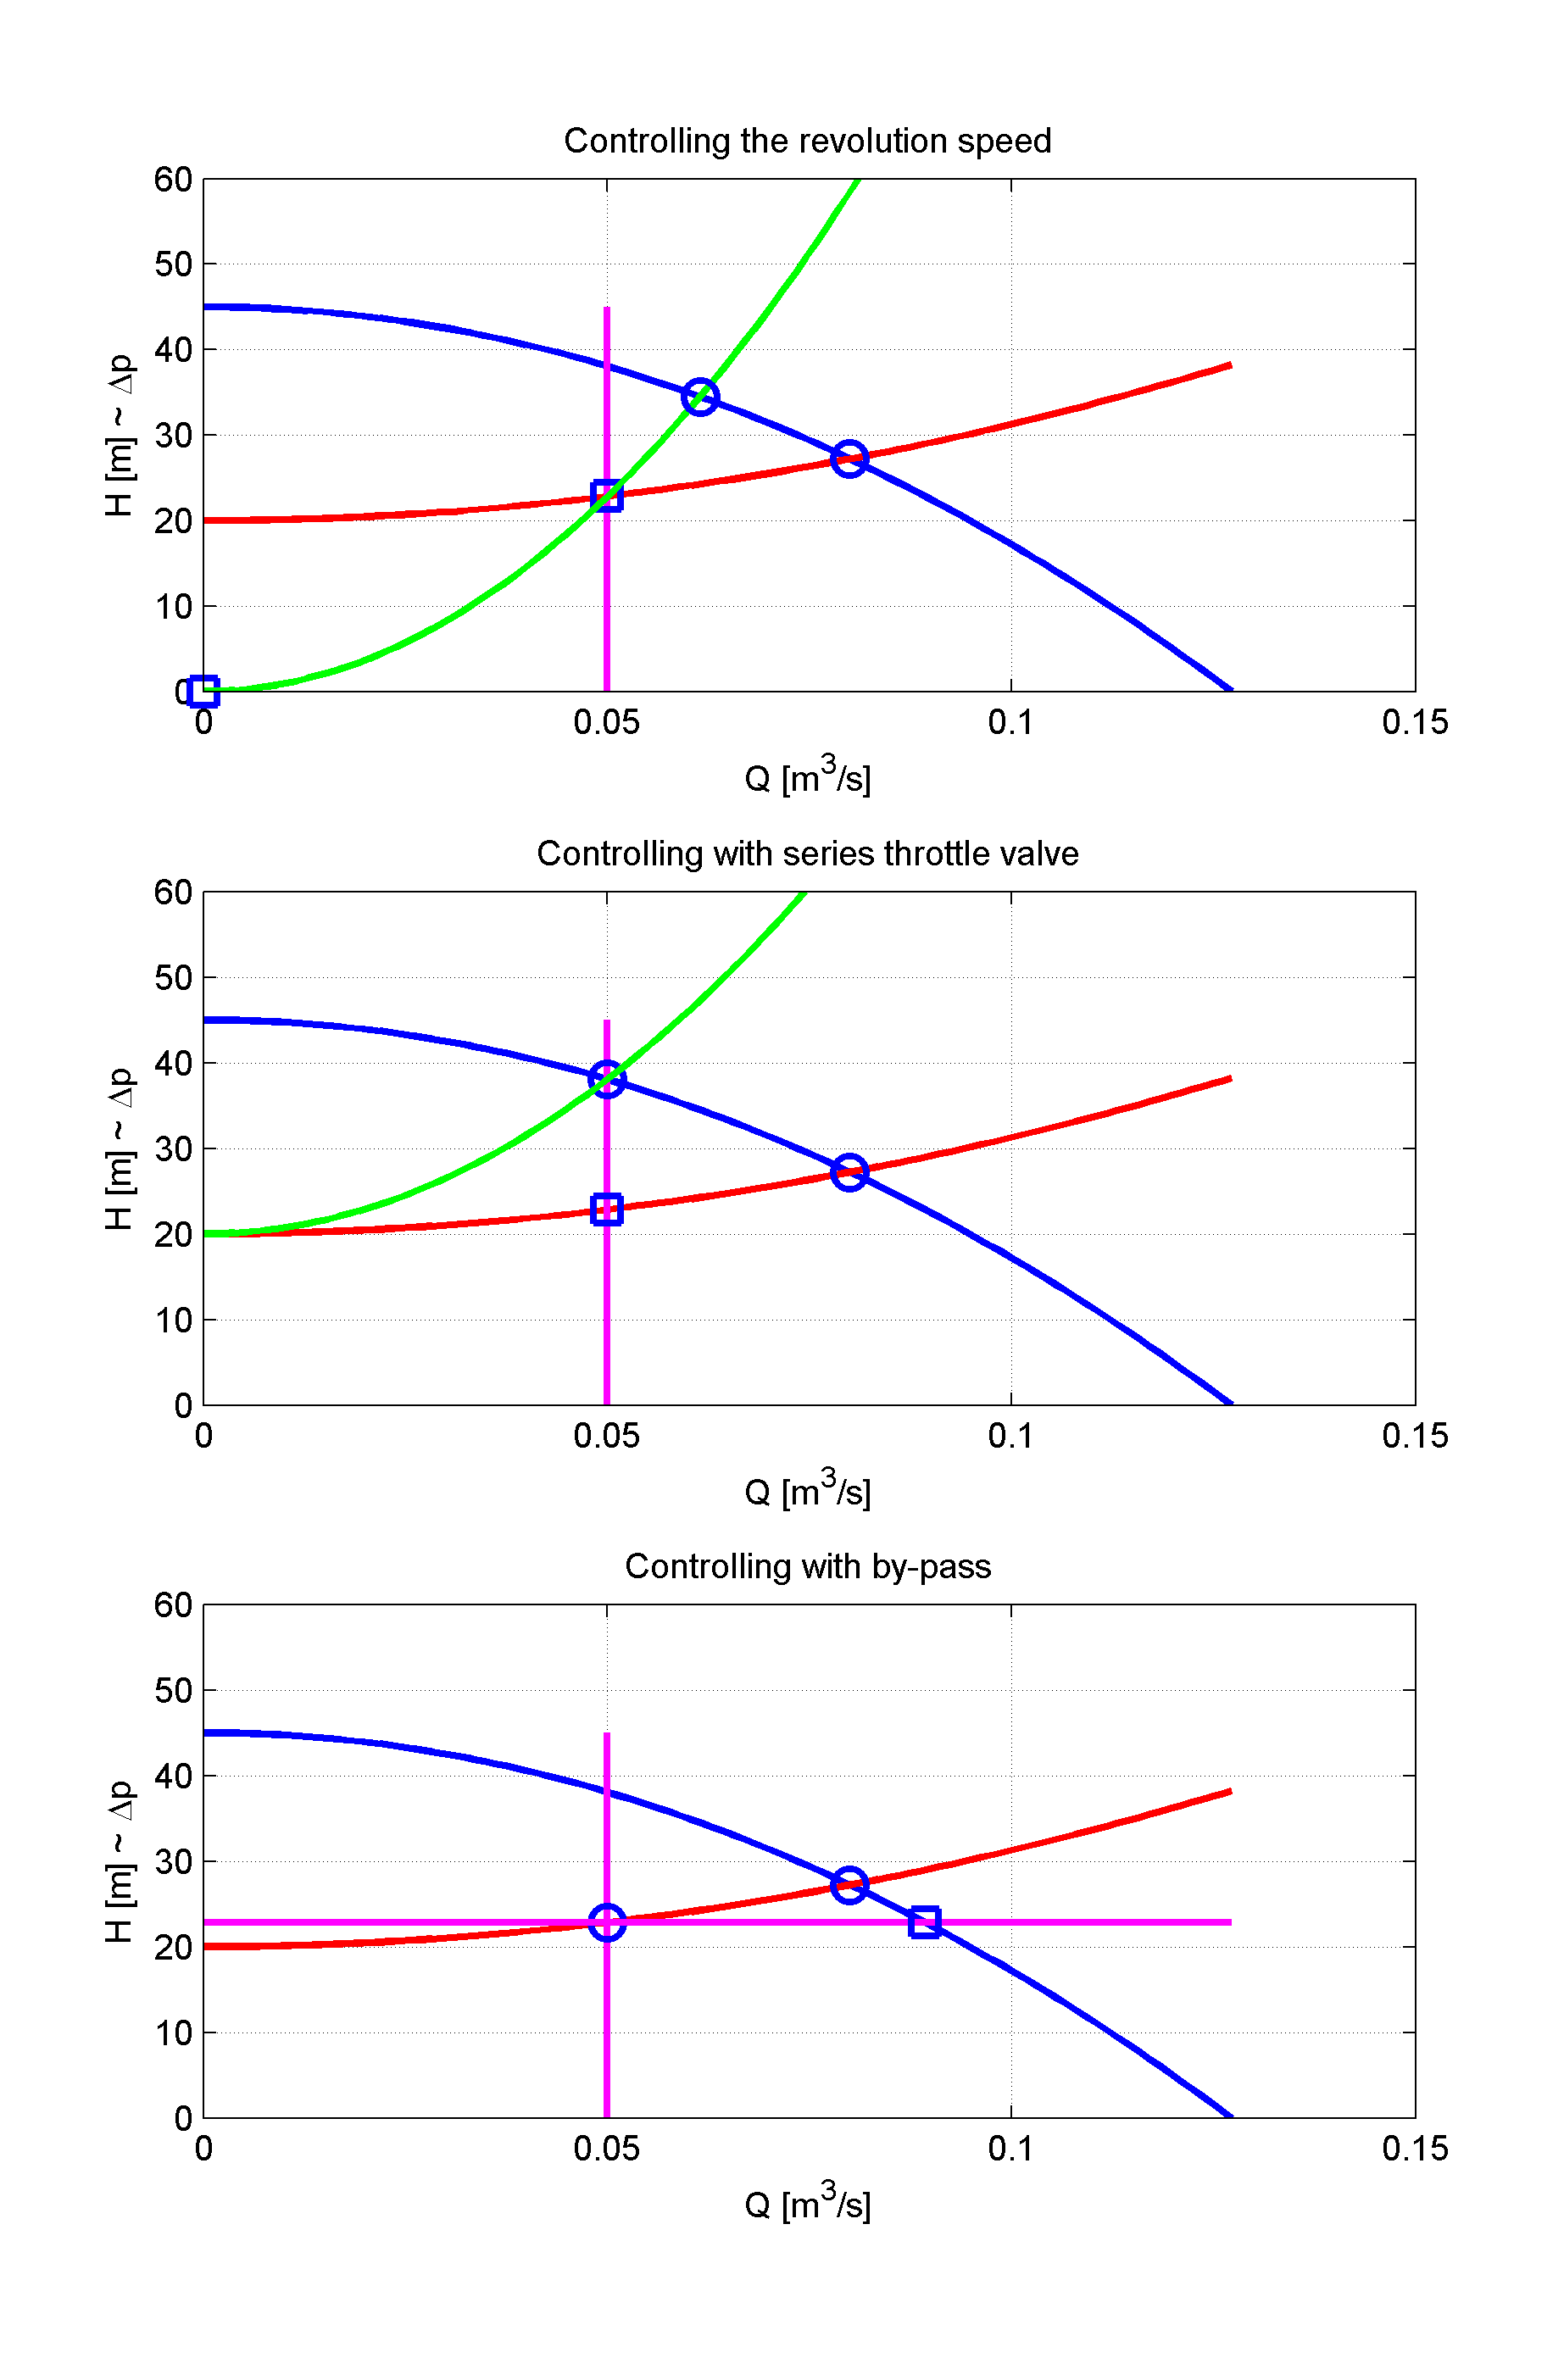
\includegraphics[width=0.7\textwidth]{Problem_solving/figs/PS_Control1.png}
\end{figure}

%%%%%%%%%%%%%%%%%%%%%%%%%%%%%%%%%%%%%%%%%%%%%%%%%%%%%%%%%%%%%%%%%%%%%%

\vspace{1cm}
\noindent {\bf Problem \thesection.\theprob}\stepcounter{prob}

A pump, whose characteristic curve is given by $H_{pump}=70-90000[s^2/m^5]Q^2$, works together with two parallel pipes. The main pipe is given by $H_1=30+100000[s^2/m^5]Q^2$. Calculate the head-flow relationship $H_2(Q)$ of the side pipe, whose opening results in a flow rate of $480[l/min]$ in the main pipe. The static head of the second side pipe is $25[m]$.

\noindent Solution: 

\begin{itemize}
\item Head of the main pipe at the prescribed flow rate: $Q_1 = 480[l/min]=0.008[m^3/s] \quad \rightarrow \quad H_1(Q_1)=36.4[m]$
%
\item The head is the same, so the flow rate of the pump is
 $H_p(Q_p)= H_1(Q_1) \quad \rightarrow \quad Q_p=\sqrt{\frac{70-36.4}{90000}}=0.0193[m^3/s]$
%
\item Thus, the flow rate on the side pipe is $Q_2=Q_p-Q_1=0.0193-0.008=0.0113[m^3/s]$
%
\item The actual characteristic of the side pipe: $H_2(Q_2)=25+aQ_2^2=36.4[m] \quad \rightarrow \quad a=\frac{36.4-25}{0.0113^2}=89279$
%
\item The solution is $H_2(Q_2)=25+89279 Q^2$.
\end{itemize}

%%%%%%%%%%%%%%%%%%%%%%%%%%%%%%%%%%%%%%%%%%%%%%%%%%%%

\vspace{1cm}
\noindent {\bf Problem \thesection.\theprob}\stepcounter{prob}

Pumps $I$ and $II$ feed pipes $1$ and $2$ shown in the figure below. Their characteristics are:
\begin{eqnarray}
	&& H_I = 45m-24900s^2/m^5Q^2 \nonumber \\
	&& H_{II} = 35m-32200s^2/m^5Q^2 \nonumber \\
	&& H_1 = 10m+4730s^2/m^5Q^2 \nonumber \\
	&& H_2 = 15m+8000s^2/m^5Q^2\nonumber
\end{eqnarray}
Find the flow rates and heads if valve $"V"$ is closed, and if it it opened. 
0.023054084926172
% (Solution: closed: $H=34.46~\mathrm{m},~Q=0.02578~\frac{\mathrm{m^3}}{\mathrm{s}}$; open:  $H=25.18\mathrm{m},~Q=0.03567~\frac{\mathrm{m^3}}{\mathrm{s}}$)
(Solution: closed: $H=31.766~\mathrm{m},~Q=0.02305~\frac{\mathrm{m^3}}{\mathrm{s}}$; open:  $H=25.18\mathrm{m},~Q=0.03567~\frac{\mathrm{m^3}}{\mathrm{s}}$)

\begin{figure}[!ht]
\centering
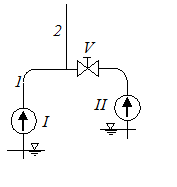
\includegraphics{Problem_solving/figs/PS_Control_Pumps.png}
\end{figure}

%%%%%%%%%%%%%%%%%%%%%%%%%%%%%%%%%%%%%%%%%%%%%%%%%%%%%%%%%%%%%%%%%%%%%%%%%%
\vspace{1cm}
\noindent {\bf Problem \thesection.\theprob}\stepcounter{prob}

Two pumps, $H_1=70m-50000s^2/m^5Q^2$ and $H_2=80m-50000s^2/m^5Q^2$ can be coupled parallel or in series. Which arrangement will deliver more liquid through the pipe $H_p=20m+25000s^2/m^5Q^2$? (Solution: in series: $Q=0.03224~\frac{\mathrm{m^3}}{\mathrm{s}},~H=46~\mathrm{m}$; in parallel: $Q=0.03818~\frac{\mathrm{m^3}}{\mathrm{s}},~H=56.44~\mathrm{m}$)

%%%%%%%%%%%%%%%%%%%%%%%%%%%%%%%%%%%%%%%%%%%%%%%%%%%%

\vspace{1cm}
\noindent {\bf Problem \thesection.\theprob}\stepcounter{prob}

Pump S, with the characteristitc curve $H_S=37-0.159Q^2$, is feeding an irrigation system consisting of parallel pipes. The units are $Q[m3/h]$ and $H[m]$. Each pipe contains at its end a sprinkler. The pipes are $20m$ long, their inner diameter is $25mm$, the friction coefficient is $0.03$. The sprinklers discharge $4 m^3/h$ water at $2 bar$ overpressure, their characteristics can be written as $H_{spr}=K_{spr}Q^2$. 

\begin{itemize}
\item Draw the sketch of the irrigation system with 3 parallel pipes!
\item How much water is discharged if only one pipe is in operation?
\item How many parallel pipes can be fed if the overpressure before the sprinklers must be $2 bar$? 
\end{itemize}

(Solution: single pipe: $Q_1 = 4.5~\frac{\mathrm{m^3}}{\mathrm{h}}$, $H=33.7~\mathrm{m}$; the pump can supply 2 pipes only)

%%%%%%%%%%%%%%%%%%%%%%%%%%%%%%%%%%%%%%%%%%%%%%%%%%%%

\vspace{1cm}
\noindent {\bf Problem \thesection.\theprob}\stepcounter{prob}

The characteristics of a pump supplying a small village with water is $H_p=70-330Q^2$. The village network is modeled by the curve $H_{cd}=25+30Q^2$ during the day while the night operation can be described by $H_{cn}=25+750Q^2$. A high water tower is attached to the delivery tube of the pump, its characteristics is $H_T=40-55|Q|Q $. Here $Q$ is positive if water flows down from the tower. The units in the formulae are [Q] = m3/s; [H] = m. Draw a sketch of the water system. Find the flow rates of the pump, village and tower both for day and night operation. Find the head of the pump both for day and night! Use a millimeter paper to draw the charasteristics curves! (Solutions: $Q_{pump}=0.33m^3/s$ and $0.29m^3/s$; $Q_{village}=0.6m^3/s$ and $0.15m^3/s$; $Q_{tower}=0.275m^3/s$ and $-0.14m^3/s$. $H_{pump}=36m$ and $41m$.)
%%%%%%%%%%%%%%%%%%%%%%%%%%%%%%%%%%%%%%%%%%%%%%%%%%%%

\vspace{1cm}
\noindent {\bf Problem \thesection.\theprob}\stepcounter{prob}

How much water is delivered by the pump $H_p=70-45000Q^2$ through the pipe system $H_s = 20+20000Q^2$ ? The flow rate must be reduced to $0.015 m^3/s$. This can be done either by throttling control or by using a by-pass control. Draw the pump-pipe-valve arrangements for both cases. How large is the hydraulic loss in the valves in the first and in the second case? The power consumption of the pump is $P_{input} = 9.4+240Q-50000Q^2$. How large is the specific energy consumption $f$ in the two cases? The units in the formulae are: $[m], [m^3/s], [kW]$. (Solution: $Q= 0.0277~\frac{\mathrm{m^3}}{\mathrm{s}}$, $P_{throttle}' = 5.2~\mathrm{kW}$, $P_{bypass}'=4.0~\mathrm{kW}$, $\mathrm{SEC}=0.237~\frac{\mathrm{kWh}}{\mathrm{m^3}}$ and $\mathrm{SEC}=0.285~\frac{\mathrm{kWh}}{\mathrm{m^3}}$, respectively.)




% SERIAL AND PARALLEL CONNECTIONS %%%%%%%%%%%%%%%%%%%%%%%%%%%%%%%%%%%%%%%%%%%%%
\section{Pumps and pipes connected in series or parallel}

In Sec.\,\ref{sec:head_discharge_curves_and_operating_point}, the determination of the operating point of a single pump working to a single hydraulic system is discussed in details, see also Fig.\,\ref{fig:SimplePumpingSystem}. In many cases, however, the flow rate or the head required by the system cannot be satisfied by a single pump efficiently. Or it is much more feasible economically (e.g., investment costs) to use several smaller pumps instead of a single much larger one. The pumps can be connected in a serial or in a parallel way. Each has its own specific application/purpose: increase primarily the produced flow rate (parallel) or increase primarily the produced head (serial). The difficulty in both cases is the determination of the equivalent characteristic curve of the coupled pumps to be able to find the operating point with the system. This is the main topic of the forthcoming sections. Figure\,\ref{fig:pump_stations_examples} shows two pump stations with pumps connected in a parallel (left-hand side) and in a serial (right-hand side) way. In more complex pump stations, the mixture of serial and parallel connections of pumps can also be found depending on the technological needs.

\begin{figure}[ht!]
	\centering
		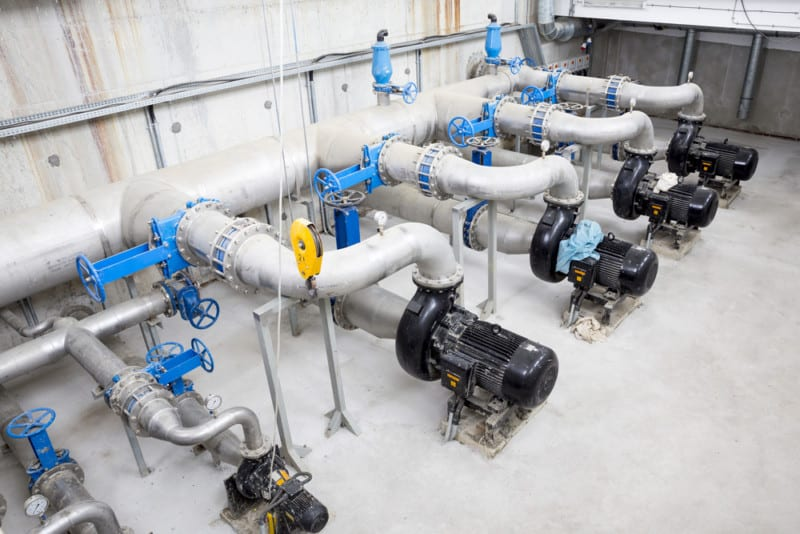
\includegraphics[height=4.5cm]{Control/Figures/Pump_Station_Parallel_Connection.jpg}
		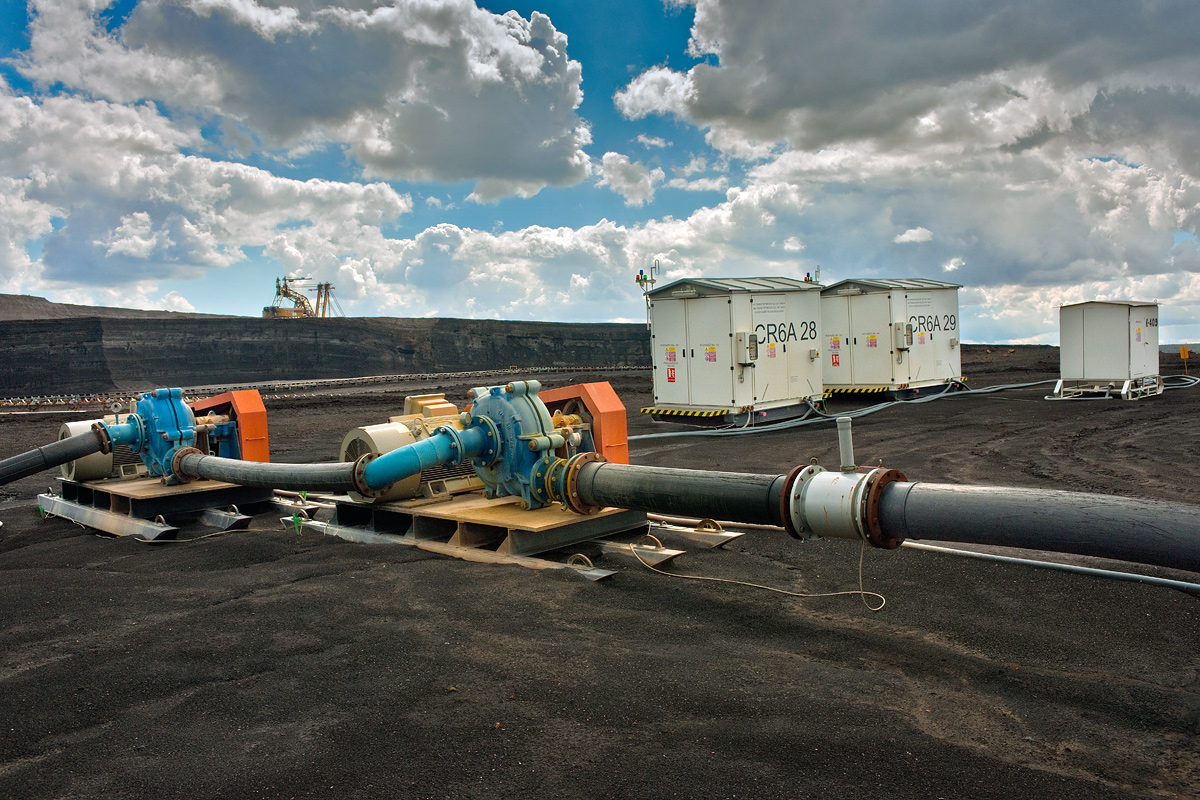
\includegraphics[height=4.5cm]{Control/Figures/Pump_Station_Serial_Connection.jpg}
	\caption{Pump stations with pumps connected in parallel (left) and in series (right).}
	\label{fig:pump_stations_examples}
\end{figure}

From the system point of view, it is also possible that a pump (or a pump station) have to provide flow rates (and head) to different systems or to a single but a complex system. In general, a system might also be composed by several subsystems built-up by a mixture of serial and parallel connections (similarly to pump stations), where each subsystem has its own characteristic curve. Again the difficulty is the derivation of an equivalent characteristic curve of the complete system.

From sizing point of view, the system of a technology or an industrial project is usually/mainly given, and the specific needs of the application drive its design. On the other hand, a pump station has to be designed according to the needs of the given hydraulic systems, which is the main focus of the sizing procedure. Naturally, it might also be possible that modifications on the system have to be carried out for efficiency reasons, and the complete design is an iterative process.

%------------------------------------------------
\subsection{Theory of serial connection} \label{sec:theory_serial_connection}
In order to introduce the basics of serial connections, consider two pumps connected in series, and working to a single system. The block diagram of such a configuration is presented in Fig.\,\ref{fig:block_diagram_serial_connection}. Due to the principle of conservation of mass, the volume flow rate (assuming incompressible flow) of the three hydraulic elements (the two pumps and the system) must be equal and denoted simply by $Q$. In contrast, the head ``production'' of the pumps are additive; that is, the overall head of the two pumps is
%
\begin{equation}
H_{p3} = H_{p1} + H_{p2}.
\end{equation}
%
Keep in mind that the head can always be regarded as pressure difference since $H_p \approx \rho g \Delta p_p$, where $\rho$ is the density and $g$ is the gravitational acceleration. In this sense, the pressure elevated by the first pump is further increased by the second pump. The system completely consumes the overall pressure difference produced by the pumps (the sum of their heads). This is the basis of operating point introduced in Sec.\,\ref{sec:head_discharge_curves_and_operating_point}. Mathematically, the solution of the algebraic equation
%
\begin{equation} \label{principle_of_serial_connection}
H_{p3}(Q) = H_{p1}(Q) + H_{p2}(Q) = H_s(Q)
\end{equation}
%
yields the flow rate $Q^o$ of the operating point.

\begin{figure}[ht!]
	\centering
		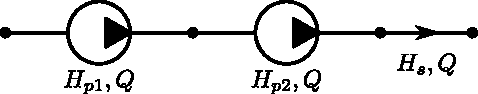
\includegraphics[height=1.25cm]{Control/Figures/Block_Diagram_Serial_Connection.pdf}
	\caption{Block diagram of two pumps connected in series, and working to a single system.}
	\label{fig:block_diagram_serial_connection}
\end{figure}

To be specific, the characteristic curves of the pumps and the system is summarized as follows
%
\begin{align}
H_{p1}(Q) &= A_{p1} - B_{p1} Q^2 = 80 -  80000 Q^2, \label{pump1_characteristic_curve_serial} \\
H_{p2}(Q) &= A_{p2} - B_{p2} Q^2 = 40 -  60000 Q^2, \label{pump2_characteristic_curve_serial} \\
H_s(Q)    &= A_s    + B_s    Q^2 = 60 + 400000 Q^2, \label{system_characteristic_curve_serial}
\end{align}
%
where the units of the head $H$ and the volume flow rate $Q$ are $\mathrm{m}$ and $\mathrm{m^3/s}$, respectively. The general form of such charateristic curves via the constants $A_i$ and $B_i$ are discussed already in Sec.\,\ref{sec:real_performance_curves_turbomachines} and Sec\,\ref{sec:head_discharge_curves_and_operating_point}; thus, it is not repeated here. The left-hand side of Fig.\,\ref{fig:example_serial_connection} represents the functions defined by Eqs.\,\eqref{pump1_characteristic_curve_serial}-\eqref{system_characteristic_curve_serial} by the black (pumps) and the red (system) curves.

\begin{figure}[ht!]
	\centering
		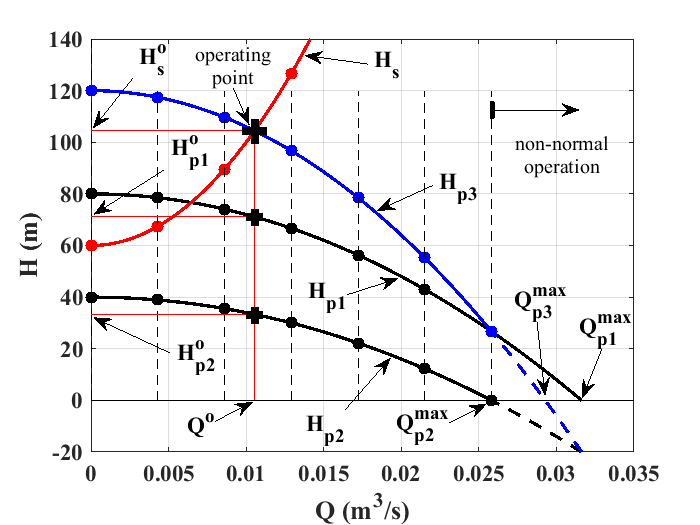
\includegraphics[width=8cm]{Control/Figures/TheorySerialConnection.png}
		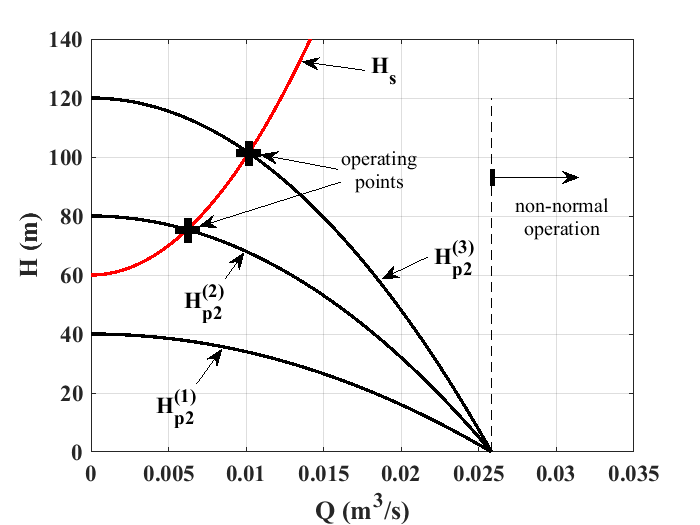
\includegraphics[width=8cm]{Control/Figures/TheorySerialConnection_SamePumps.png}
	\caption{Left panel: characteristic curves and the determination of the operating point of the hydraulic system presented in Fig.\,\ref{fig:block_diagram_serial_connection}. Right panel: effect of using multiple identical pumps connected in series on the operating point (with the same system).}
	\label{fig:example_serial_connection}
\end{figure}

The first task is to unite the two characteristic curves of the pumps in order to determine the operating point. According to Eq.\,\eqref{principle_of_serial_connection}, it is simply the summary of the heads. As the characteristic curves are already expressed for the heads in Eqs.\,\eqref{pump1_characteristic_curve_serial}-\eqref{system_characteristic_curve_serial}, the overall characteristic curve of the two pumps can be obtained analytically very easily:
%
\begin{equation}
\begin{split}
H_{p3}(Q) &= H_{p1}(Q) + H_{p2}(Q), \\
          &= 80 - 80000 Q^2 + 40 - 60000 Q^2, \\
		  &= 120 - 140000 Q^2,
\end{split}
\end{equation}
%
shown by the blue curve in Fig.\,\ref{fig:example_serial_connection} left. The operating point of the whole hydraulic system is at the intersection of the blue and the red curves marked by the big black cross. Numerically, the volume flow rate of the operation point $Q^o$ can be calculated by equating the two characteristic curves:
%
\begin{equation}
\begin{split}
         H_{p3}(Q^o) &= H_{s}(Q^o), \\
120 - 140000 (Q^o)^2 &= 60 + 400000 (Q^o)^2, \\
		          60 &= 540000 (Q^o)^2, \\
			     Q^o &= \sqrt{\frac{60}{540000}} = 0.01054\,\mathrm{\frac{m^3}{s}}.
\end{split}
\end{equation}
%
The head of the system can be calculated by substituting the flow rate of the operating point $Q^o$ into Eq.\,\eqref{system_characteristic_curve_serial}:
%
\begin{equation} \label{principle_of_serial_connection}
H_s^o = A_s + B_s Q^2 = 60 + 400000 (Q^o)^2 = 104.4\,\mathrm{m}.
\end{equation}
%
since the same volume flow rate $Q^o$ flows through both pumps, their individual operating points are at the crossings of their characteristic curves with the red vertical line at $Q^o$, see the small black crosses in the left-hand side of Fig.\,\ref{fig:example_serial_connection}. Again, the heads of the operating points of the pumps can be obtained by substitution:
%
\begin{align}
H_{p1}^o &= A_{p1} - B_{p1} Q^2 = 80 - 80000 (Q^o)^2 = 77.1\,\mathrm{m}, \\
H_{p2}^o &= A_{p2} - B_{p2} Q^2 = 40 - 60000 (Q^o)^2 = 33.3\,\mathrm{m}.
\end{align}
%
With the above-described calculations, all the properties (heads and flow rates) of all the elements of the whole hydraulic system could be obtained, see also the labels in the left-hand side of Fig.\,\ref{fig:example_serial_connection} pointing to the projections to the horizontal and vertical axes by the thin red lines.

In some cases, it may happen that the characteristic curves are not given in an analytical form; for instance, only a graphical curve is given in an old catalogue, or only some measured points are available. In this case, there is an alternative, graphical solution to approximate the operating point. The first step is the division of the volume flow rate range into a discrete set of values represented by the vertical dashed lines in Fig.\,\ref{fig:example_serial_connection} left. Second, evaluate the characteristic curves of the pumps and the system at these flow rate values (see the black and red dots). This process may already be done by a measurement. Next, the equivalent characteristic curve of the two pumps can be obtained by summing the values of the heads of the black dots at a given dashed line and mark the corresponding (blue) point on the same dashed line. The result is the series of blue dots in Fig.\,\ref{fig:example_serial_connection} left. Drawing (by hand) the approximated characteristic curves through the calculated dots, the intersection of the blue and the red curves will define the estimated operating point as usual. Finally, the projections via the thin red lines defines the values of the operating heads and flow rates of the individual pumps and the system.

At this point, some important remarks need to be done. First of all, the addition of characteristic curves in a serial way is not a speciality for pumps. Basically, any kinds of characteristic curves can be added together (pump-pump, pump-system, system-system). One of the issues one has to keep in mind is the addition in terms of the heads; namely, addition vertically, e.g., along the thin dashed lines presented in Fig.\,\ref{fig:example_serial_connection} left. Moreover, adding characteristic curves of a pump and a system together, the signs of the heads (production or consumption) have to be taken into account; that is, the head of the system must be subtracted from the head of the pump (instead of adding them together). This is important for complex hydraulic connections with multiple pumps and subsystems. For an example of an addition of a pump-system characteristic curve, the reader is referred to Sec.\,\ref{sec:operation_point_complex_connections}.

Second, the highest volume flow rate the second pump can provide at zero head ($H=0$, thin black horizontal line in Fig.\,\ref{fig:example_serial_connection} left) is $Q_{p2}^{max}=0.0258\,\mathrm{m^3/s}$. The zero head means an approximately zero pressure difference between the two sides of the pump; that is, the pump has to convey fluid against zero resistance. Thus, the pump has the highest possible volume flow rate at this condition. Naturally, this is an extreme limit case. Observe that for volume flow rates higher than the maximum value ($Q>Q_{p2}^{max}$), the characteristic curve of the second pump has a \textit{negative head} depicted by the continuation of the corresponding black curve with its dashed extension. Thus, at a flow rate higher than $Q_{p2}^{max}$, the second pump becomes a resistance or a ``consumer'' of the head instead of a producer. The negative head means that there is a pressure prop at the pump, which must be satisfied, e.g., by the first pump. Practically, this means that the first pump pushes the volume flow rate through the second pump. The consequence is that the fluid transport would be higher by taking the second pump out of the system. This can also be seen from the limit case of $H=0$, where the continuation of the blue curve up to the horizontal axis yields a lower maximum flow rate ($Q_{p3}^{max}=0.0293\,\mathrm{m^3/s}$) than the one of the first pump alone $Q_{p1}^{max}=0.0316\,\mathrm{m^3/s}$. Definitely, operation of the system shown in Fig.\,\ref{fig:block_diagram_serial_connection} with a flow rate of $Q>Q_{p2}^{max}$ is \textit{not} a normal design, and should be avoided.

Third, using identical pumps (which is quite common in practice), the calculation of the equivalent characteristic curve of the pumps is greatly simplified. Using $n$ number of pumps of the second type that are connected in series, the equivalent characteristic curve can be written as
%
\begin{equation}
H_{p2}^{(n)} = n A_{p2} - n B_{p2} Q^2 = n 40 - n 60000 Q^2.
\end{equation}
%
For $n=1,2$ and $3$, the corresponding characteristic curves are presented in Fig.\,\ref{fig:example_serial_connection} right by the black curves. Note that in this case, the curves (for all $n$) coincide at the horizontal axis ($H=0$) having the same maximum flow rate as a limit case of the normal operation.

Fourth, from Fig.\,\ref{fig:example_serial_connection}, it is clear that the serial connection of pumps increase primarily the available head for the system. It is apparent also from the summing technique. However, the increase of the head is \textit{non-linear} with the number of pumps $n$ (even employing identical pumps). Considering the case in the right-hand side of Fig.\,\ref{fig:example_serial_connection}, with a single pump, there is no valid operating point in the normal operation regime as a single pump cannot provide enough head to overcome the static head of the system ($A_s=60\,\mathrm{m}$). With two or three pumps, there are operating points (intersections with the red curves) marked by the black crosses. Parenthetically, if the required flow rate is $Q_r=0.01\,\mathrm{m^3/s}$, the application of at least three pumps is necessary. In order to highlight the non-linear characteristics of the operating point as a function of $n$, let us summarize the corresponding values of $H^o$ and $Q^o$ in Tab.\,\ref{tab:summary_oprating_points_serial_connection}. In case of a linear relationship of the values of $H^o$ as a function of $n$, the ratio of the heads would be $3/2$ by increasing the number of pumps from $n=2$ to $3$. In contrast, the numbers in Tab.\,\ref{tab:summary_oprating_points_serial_connection} do \textit{not} support this hypothesis:
%
\begin{equation}
\frac{ H_{p2}^{(3)} }{ H_{p2}^{(2)} } \Bigg)_{op.} = \frac{101.5}{75.4} = 1.35 < \frac{3}{2} = 1.5.
\end{equation}
%
The reason is that the addition of the characteristic curves of the pumps takes place ``purely'' vertically; meanwhile, the operating point moves along the characteristic curve of the system (red curve). This finding also holds for the volume flow rates (check the numbers in Tab.\,\ref{tab:summary_oprating_points_serial_connection}), and the following rule-of-thumb can be formulated: \textbf{doubling the number of the pumps does NOT double the head and/or the volume flow rate}.

\begin{table}[ht!]
\caption{Summary of the values of the heads $H^o$ and volume flow rates $Q^o$ of the operating points shown in the right-hand side of Fig.\,\ref{fig:example_serial_connection} by the black crosses.}
	\label{tab:summary_oprating_points_serial_connection}
	\centering
		\begin{tabular}{c|cc}
		 $n$ & $H^o (\mathrm{m})$ & $Q^o (\mathrm{m^3/s})$ \\ \hline \hline
		 1   & -                  & -        \\
		 2   & 75.4               & 0.006203 \\
		 3   & 101.5              & 0.01018  \\
		\end{tabular}
\end{table}

%------------------------------------------------
\subsection{Theory of parallel connection}
Continue our discussion with the basics of the parallel connection. Similarly, as in the case in Sec.\,\ref{sec:theory_serial_connection}, consider two pumps, which are working to a single system. However, now they are connected in parallel. The corresponding block diagram is shown in Fig.\,\ref{fig:block_diagram_parallel_connection}. The conservation principle of mass means that the sum of the volume flow rates of the pumps $Q_{p3}$ is equal to the volume flow rate of the system:
%
\begin{equation} \label{conservation_of_mass_parallel_connection}
Q_{p3} = Q_{p1} + Q_{p2} = Q_s.
\end{equation}
%
Moreover, the heads of the pumps must be the same ($H_{p1}=H_{p2}$) as their suction and pressure sides are connected; that is, the pressure difference between the two sides of both pumps is equal. The pumps deliver, e.g., water from the same reservoir to the same system. Keep in mind that pressure difference is proportional to the head of the pumps. The consideration mentioned above implies that the summing procedure of the characteristic curves of the pumps must be done in terms of the flow rate (horizontally) instead of in terms the heads (vertically), compare also with the case in Sec.\,\ref{sec:theory_serial_connection}. Without the details of the derivation at the moment, let us denote this combined characteristic curve by $H_{p3}(Q_{p3})$. Now, the operating point of the complete hydraulic system can be determined by equating the characteristic curves of the combined pumps and the system:
%
\begin{equation} \label{operating_point_of_parallel_connection}
H_{p3}(Q_{p3}) = H_{p3}(Q_s) = H_s(Q_s).
\end{equation}
%
Again, the solution of Eq.\,\eqref{operating_point_of_parallel_connection} yields the flow rate $Q^o$ of the operating point. Note that $H_{p1}=H_{p2}=H_s$ during an operation of a hydraulic system shown in Fig.\,\ref{fig:block_diagram_parallel_connection}; thus, these heads are denoted simply by $H$.

\begin{figure}[ht!]
	\centering
		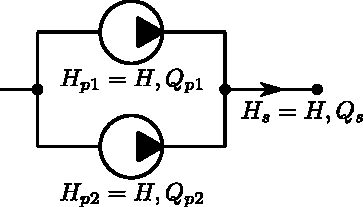
\includegraphics[height=2.75cm]{Control/Figures/Block_Diagram_Parallel_Connection.pdf}
	\caption{Block diagram of two pumps connected in parallel, and working to a single system.}
	\label{fig:block_diagram_parallel_connection}
\end{figure}

Let us continue the discussion again with a specific example. The characteristic curves of the hydraulic elements presented in Fig.\,\ref{fig:block_diagram_parallel_connection} are
%
\begin{align}
H_{p1}(Q_{p1}) &= A_{p1} - B_{p1} Q_{p1}^2 = 80 - 80000 Q_{p1}^2, \label{pump1_characteristic_curve_parallel} \\
H_{p2}(Q_{p2}) &= A_{p2} - B_{p2} Q_{p2}^2 = 60 - 70000 Q_{p2}^2, \label{pump2_characteristic_curve_parallel} \\
H_s(Q_s)       &= A_s    + B_s    Q_s^2    = 15 + 10000 Q_s^2.    \label{system_characteristic_curve_parallel}
\end{align}
%
These curves are also drawn in the left-hand side of Fig.\,\ref{fig:example_parallel_connection} by the black (pumps) and the red (system) curves, see the corresponding labels as well.

\begin{figure}[ht!]
	\centering
		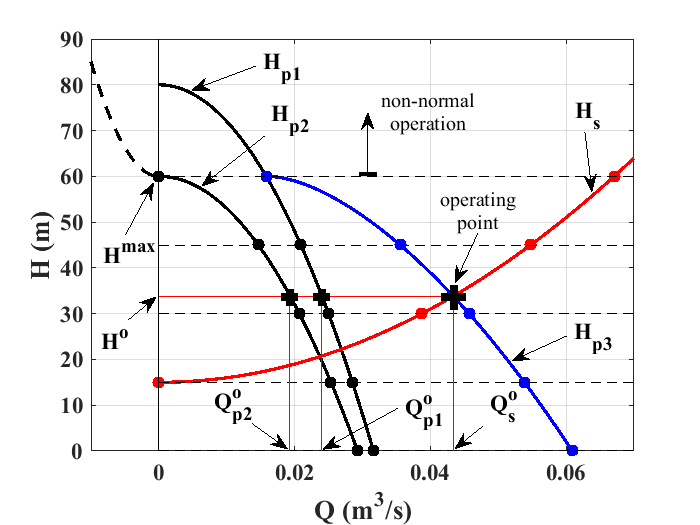
\includegraphics[width=8cm]{Control/Figures/TheoryParallelConnection.png}
		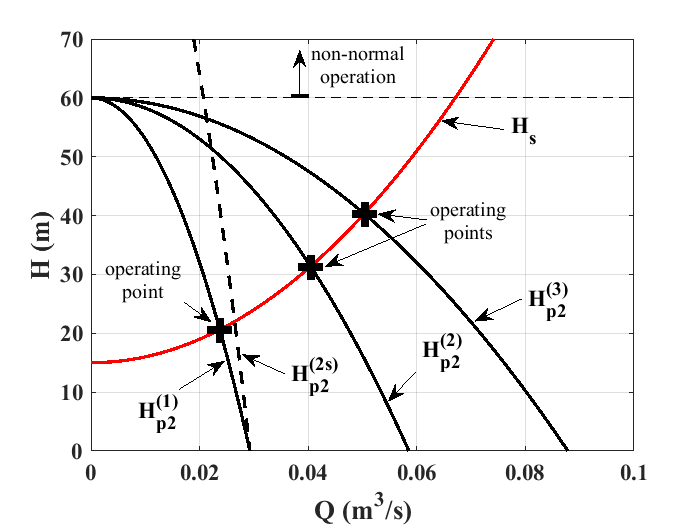
\includegraphics[width=8cm]{Control/Figures/TheoryParallelConnection_SamePumps.png}
	\caption{Left panel: characteristic curves and the determination of the operating point of the hydraulic system presented in Fig.\,\ref{fig:block_diagram_parallel_connection}. Right panel: effect of using multiple identical pumps connected in parallel on the operating point (with the same system).}
	\label{fig:example_parallel_connection}
\end{figure}

Similarly, as in the case of the serial connection, the first step is the determination of the combined characteristic curve of the pumps. According to Eq.\,\eqref{conservation_of_mass_parallel_connection}, the summation of the curves have to be carried out in terms of the volume flow rates; thus, Eqs.\,\eqref{pump1_characteristic_curve_parallel}-\eqref{pump2_characteristic_curve_parallel} needs to be rearranged to the flow rates. These inverse characteristic curves read as
%
\begin{align}
Q_{p1}(H) &= \sqrt{ \frac{A_{p1}-H}{B_{p1}} } = \sqrt{ \frac{80-H}{80000} }, \label{pump1_inverse_characteristic_curve_parallel} \\
Q_{p2}(H) &= \sqrt{ \frac{A_{p2}-H}{B_{p2}} } = \sqrt{ \frac{60-H}{70000} }. \label{pump2_inverse_characteristic_curve_parallel}
\end{align}
%
Keep in mind that $H_{p1}=H_{p2}=H$. The invesre function of the combined characterisctic curve is simply the addition of Eq.\,\eqref{pump1_inverse_characteristic_curve_parallel} and \eqref{pump2_inverse_characteristic_curve_parallel}:
%
\begin{equation} \label{combined_characteristic_curve_parallel_connection}
Q_{p3}(H) = Q_{p1}(H) + Q_{p2}(H) = \sqrt{ \frac{A_{p1}-H}{B_{p1}} } + \sqrt{ \frac{A_{p2}-H}{B_{p2}} } = \sqrt{ \frac{80-H}{80000} } + \sqrt{ \frac{60-H}{70000} }.
\end{equation}
%
Unfortunately, for general values of $A_{p1}$, $A_{p2}$, $B_{p1}$ and $B_{p2}$, there are no simple means to rearrange Eq.\,\eqref{combined_characteristic_curve_parallel_connection} to the head $H$; that is, to retrieve the ``non-inverse'' combined characteristic curve $H_{p3}(Q_{p3})$. In Fig.\,\ref{fig:example_parallel_connection} left, the function $H_{p3}(Q_{p3})$ is shown as a blue curve, and it is calculated numerically in MATLAB using the built-in non-linear algebraic equation solver \textit{fzero}. If software environments are not available to carry out detailed numerical calculations, the graphical approach introduced in Sec.\,\ref{sec:theory_serial_connection} is still a viable option. The only difference is that the curves are summarized in terms of the flow rates (instead of in terms of the head) highlighted by horizontal thin dashed lines in the left-hand side of Fig.\,\ref{fig:example_parallel_connection}. That is, the addition of the flow rates of two black dots yields a blue dot, where all the three dots are lying on the same dashed line. This is a quick hand-made approximation of the characteristic curves.

As usual, the operating point of the hydraulic system is at the intersection of the blue and the red curve presented by the big black cross. Its volume flow rate $Q^o=0.0434\,\mathrm{m^3/s}$ and head $H^o=33.8\,\mathrm{m}$ can be obtained by the projection of the operating point to the horizontal and vertical axes, respectively; see also the corresponding thin red lines in Fig.\,\ref{fig:example_parallel_connection} left. Since the blue curve is only a fine series of numerically calculated points, the location of the above-determined operating point is also given only numerically. However, by substituting the volume flow rate of the operating point into the characteristic curve of the system, one can double-check the results:
%
\begin{equation}
H_s^o = A_s + B_s Q^2 = 15 + 10000 (Q^o)^2 = 33.836\,\mathrm{m},
\end{equation}
%
which agrees well with the aforementioned value. Since both pumps operate at the same level of head ($H_{p1}^o=H_{p2}^o=H_s^o=H^o$), their operating volume flow rate can be obtained by a simple substitution into Eqs.\,\eqref{pump1_inverse_characteristic_curve_parallel}-\eqref{pump2_inverse_characteristic_curve_parallel}:
%
\begin{align}
Q_{p1}^o &= \sqrt{ \frac{A_{p1}-H^o}{B_{p1}} } = \sqrt{ \frac{80-33.8}{80000} } = 0.0240\,\mathrm{m^3/s}, \\
Q_{p2}^o &= \sqrt{ \frac{A_{p2}-H^o}{B_{p2}} } = \sqrt{ \frac{60-33.8}{70000} } = 0.0193\,\mathrm{m^3/s},
\end{align}
%
see the projections by the red lines again. With the above-described method, all the important details of the operating conditions of the system and both pumps are determined.

The majority of the remarks pointed out in Sec.\,\ref{sec:theory_serial_connection} is valid here as well. Namely, the addition of characteristic curves in a parallel way is not a special property for pumps. Any type of characteristic curves can be summarized horizontally in terms of the flow rate (pump-pump, pump-system, system-system). However, in the case of pump-system configuration, the flow rate of the system must be substracted (instead of added) from the flow rate of the pump. This is necessary to properly take into account that the pump ``provides'' flow rate while the system ``consumes'' flow rate.

In case of parallel connection, there is also a non-normal operation regime presented by the uppermost thin dashed line in the left panels of Fig.\,\ref{fig:example_parallel_connection}. Above this limit, the volume flow rate of the second pump becomes negative (dashed thick continuation of its characteristic curve); that is, there is a backflow in the second pump. In such a situation, the first pump circulates some amount volume flow rate in the parallel loop. This design should be avoided.

In a special case, where the same pumps connected in parallel, the combined characteristic curve can be derived analytically. Similarly to Eq.\,\eqref{combined_characteristic_curve_parallel_connection}, the inverse characteristic curve of $n$ number of pumps of the second type (connected in parallel) can be derived as
%
\begin{equation}
Q_{p2}^{(n)} = n Q_{p2} = n \sqrt{ \frac{A_{p2}-H}{B_{p2}} } = n \sqrt{ \frac{60-H}{70000} }.
\end{equation}
%
This can easily be rearranged to the head:
%
\begin{equation}
H_{p2}^{(n)} = A_{p2} - \frac{B_{p2}}{n^2} Q^2  = 60 - \frac{70000}{n^2} Q^2.
\end{equation}
%
The characteristic curves for $n=1$, $2$ and $3$ are depicted in the right-hand side of Fig.\,\ref{fig:example_parallel_connection} by the solid black curves. The black crosses present all the operating points (intersections with the red system curve). As an interesting comparison, the case of two pumps connected in series ($H_{p2}^{(2s)}$) is also shown in this figure as a dashed thick black curve. It is clear that in the serial case, for such a system characteristic curve, the alteration of the operating point is marginal compared to the usage of a single pump ($H_{p2}^{(1)}$). \textit{That is, we doubled the investment cost without any practical consequence}.

Finally, let us emphasize the non-linear nature of the parallel connection. The values of the volume flow rates and the heads of the three operating points presented by the crosses in Fig.\,\ref{fig:example_parallel_connection} are summarized in Tab.\,\ref{tab:summary_oprating_points_parallel_connection}. The results strengthen our previous conclusion: \textbf{doubling or tripling the number of the pumps does NOT double or triple the flow rate and/or the head}.

\begin{table}[ht!]
\caption{Summary of the values of the heads $H^o$ and volume flow rates $Q^o$ of the operating points shown in the right-hand side of Fig.\,\ref{fig:example_parallel_connection} by the black crosses.}
	\label{tab:summary_oprating_points_parallel_connection}
	\centering
		\begin{tabular}{c|cc}
		 $n$ & $H^o (\mathrm{m})$ & $Q^o (\mathrm{m^3/s})$ \\ \hline \hline
		 1   & 40.3               & 0.05031 \\
		 2   & 31.4               & 0.04044 \\
		 3   & 20.7               & 0.02371 \\
		\end{tabular}
\end{table}

%------------------------------------------------
\subsection{Operating point of complex connections} \label{sec:operation_point_complex_connections}

%------------------------------------------------
\subsection{Problems}

%%%%%%%%%%%%%%%%%%%%%%%%%%%%%%%%%%%%%%%%%%%%%%%%%%%%

\noindent {\bf Problem \thesection.\theprob}\stepcounter{prob}

The performance curve of a pump is $H_p = 70-10000\,Q^2$. This pump is connected to two pipe systems with characteristic curves $H_{s1} = 5000\,Q^2+10$ and $7500\,Q^2+15$. In these formulae, the head is in meters, and the unit of the volumetric flow rate is $\frac{\mathrm{m^3}}{\mathrm{s}}$. Find the operation point, if the two pipe systems are connected (a) in series, or (b) in parallel to the pump. Draw the performance curves in both cases!

Solution: when the pipe systems are in series connection, the volumetric flow rate through them is the same, and in the calculation of the performance curves, the heads are summed at each volumetric flow rate. This means:
\begin{equation*}
H_{s,ser} = H_{s1} + H_{s2} = 12500\,Q^2+25.
\end{equation*}
In the operation point, the head of the pump equals the head required by the system:

\begin{align*}
& H_{s,ser} = H_p, \\
& 12500\,Q^2+25=70-10000\,Q^2,\\
& Q_{ps} = \sqrt{\frac{45}{22500}} = 0.04472~\frac{\mathrm{m^3}}{\mathrm{s}}, \\
& H = H_p(Q_{ps}) = H_{s,ser} = 70 - 10000\cdot 0.04472^2 = 50~\mathrm{m}.
\end{align*}

When the two pipe systems are connected in parallel, the pressure drop/head is the same on them, while their volumetric flow rates are different. In this case, to calculate the characteristic curve of the total system, the volumetric flow rates should be summed at each head. To do this,  we need to rearrange the performance curves to be functions of the head:
\begin{align*}
& H_p = 70-10000\,Q^2 \rightarrow Q_p = \frac{\sqrt{70-H}}{100} \\
& H_{s1} = 5000\,Q^2+10 \rightarrow Q_{s1} = \frac{\sqrt{2}\,\sqrt{H-10}}{100} \\
& H_{s2} = 7500\,Q^2+15 \rightarrow Q_{s2} = \frac{\sqrt{3}\,\sqrt{H-15}}{150} .
\end{align*}
Note that the expressions above are only valid for a certain $H$ interval, since the argument of the square root function cannot be negative. Calculating the sum of the two parallel pipes, then equating the pump and the system, solving for $H$, the operating point can be identified:
\begin{align*}
& Q_{s,par} = Q_{s1} + Q_{s2} = \frac{\sqrt{2}\,\sqrt{H-10}}{100}+\frac{\sqrt{3}\,\sqrt{H-15}}{150}  = Q_p = \frac{\sqrt{70-H}}{100}\\
& H =  20.03~\mathrm{m}, \\
& Q = 0.07069~\frac{\mathrm{m^3}}{\mathrm{s}}.
\end{align*}

The performance curves are displayed in Figure \ref{fig_example1}.

\begin{figure}[!htb]
\centering
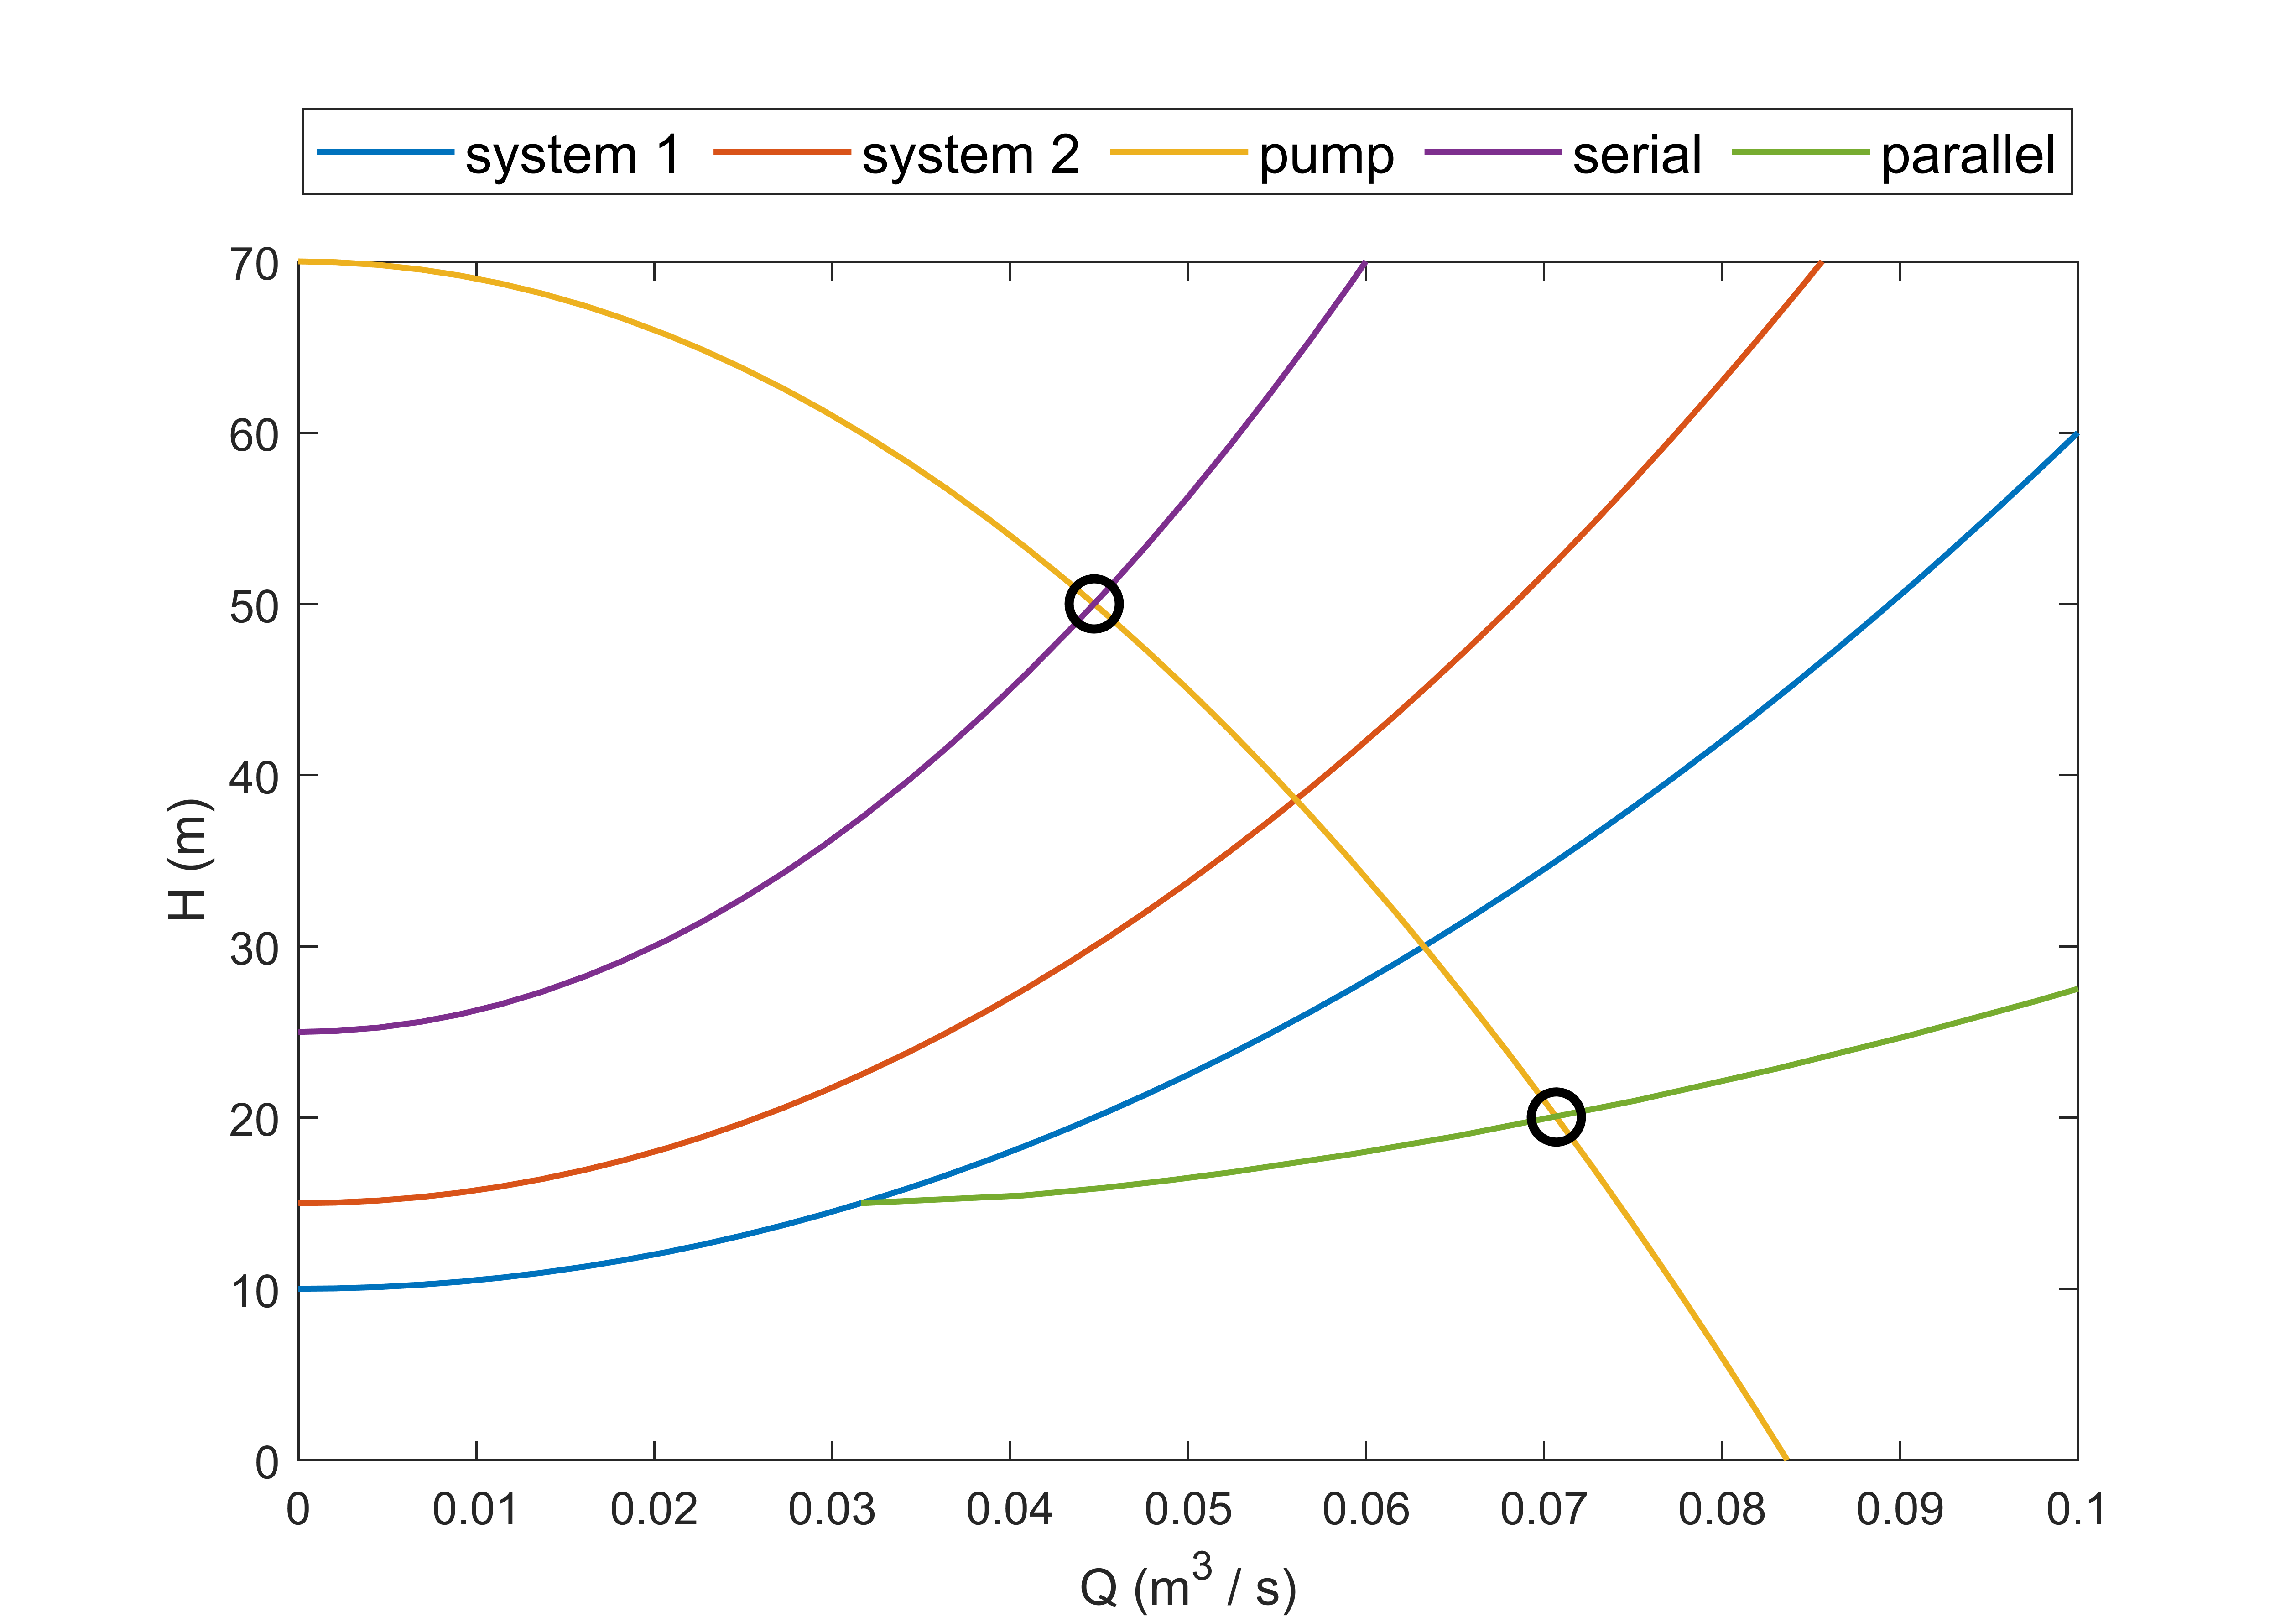
\includegraphics[width=0.8\textwidth]{figs/problem_5_par_1.png} 
\caption{ Performance curves of the problem. The circles denote the operation points.}
\label{fig_example1}
\end{figure}

%%%%%%%%%%%%%%%%%%%%%%%%%%%%%%%%%%%%%%%%%%%%%%%%%%%%

\vspace{1cm}
\noindent {\bf Problem \thesection.\theprob}\stepcounter{prob}

Two pumps, with performance curves $H_{p1} = 50 - 30000\cdot Q^2$ and $H_{p2} =  40 - 20000\cdot Q^2$ are conveying water through a pipe system that's characteristic curve is $H_s = 3 + 7250\cdot Q^2$. Find the operating points if the two pump are connected (a) in series or (b) in parallel! (Solution: $H_{ser} = 14.02~\mathrm{m}$, $Q_{ser} = 0.03898~\frac{\mathrm{m^3}}{\mathrm{s}}$, $H_{par} = 25.43~\mathrm{m}$, $Q_{par} = 0.05562~\frac{\mathrm{m^3}}{\mathrm{s}}$)

%%%%%%%%%%%%%%%%%%%%%%%%%%%%%%%%%%%%%%%%%%%%%%%%%%%%
%peldatar 6.1

\vspace{1cm}
\noindent {\bf Problem \thesection.\theprob}\stepcounter{prob}

A pump that's performance curve is $H_I (\mathrm{m}) = 70 - 50000 \frac{\mathrm{s^2}}{\mathrm{m^5}} Q^2$, conveys water through a pipe system with characteristic curve $H_s (\mathrm{m}) = 20 + 10000 \frac{\mathrm{s^2}}{\mathrm{m^5}} Q^2$. Find the volumetric flow rate! The volumetric flow rate is increased to $Q=0.032~\frac{\mathrm{m^3}}{\mathrm{s}}$, using a second pump with performance curve $H_{II} (\mathrm{m}) = 80 - 50000 \frac{\mathrm{s^2}}{\mathrm{m^5}} Q^3$. The operating point of the system is set by a throttle valve at the pressure side. How would the loss power be smaller: if the two pumps were connected in series or in parallel? (Solution: $Q=0.0285~\frac{\mathrm{m^3}}{\mathrm{s}}$, $P_{ser}' = 5.45~\mathrm{kW}$, $P_{par}' = 9.88~\mathrm{kW}$)

%%%%%%%%%%%%%%%%%%%%%%%%%%%%%%%%%%%%%%%%%%%%%%%%%%%%

\vspace{1cm}
\noindent {\bf Problem \thesection.\theprob}\stepcounter{prob}

Two pump operate in parallel. The performance curve of the first pump and it's pressure side pipeline is the following: $H_{pI} = 40 - 0.17Q^2$, $H_{s,I} = 5 + 0.4Q ^2$; the data for the second pipe is $H_{pII} = 27 - 0.135Q^2$, $H_{s,II} = 0.8Q ^2$. The head in in meters, and the unit of the volumetric flow rate is $\frac{\mathrm{m^3}}{h}$. These two pipes are joined, and convey water through a third pipeline with characteristic curve $H_{s,III} = -3 + 0.63Q ^2$. Find the operating point! (Solution: $Q = 6.473~\frac{\mathrm{m^3}}{h}$, $H=23.4~\mathrm{m}$.)

% WATER HAMMER, HYDRAULIC TRANSIENTS %%%%%%%%%%%%%%%%%%%%%%%%%%%%%%%%%%%%%%%%%%
\section{Water hammer, hydraulic transients}

Up to this point, turbomachinery is discussed from a stationary operation point of view. Such a discussion have its own right, since most of its lifetime, an installation operates in steady-state fashion. One of the main reasons is the efficiency: a device is usually designed to operate efficiently over a specific parameter range around the designed operation point. Thus, a significant deviation from this optimal point can considerably increase the operating costs or needs expensive additional equipment to overcome this issue. The previous sections of this chapter are devoted to this problem. Moreover, transient operations are usually causing greater wear of the elements of a device, which might result in a lower lifetime and additional maintenance and investment costs.

We shall see in this section that transient phenomenon in a hydraulic system also plays a significant role, although its timespan is usually many orders of magnitude smaller than steady-state operations. The starting and stopping of hydraulic machinery are two natural examples. The phenomenon discussed in this section is the generated pressure surge or wave by the sudden closure of a valve. This pressure wave, having even tenths of bars peak value, can cause major problems; for instance, the rupture or the collapse of a pipe. Transients can also be generated in a domestic environment by the sudden close (e.g., within a fraction of a second if it is allowed by design) of the faucet in the bathroom or the kitchen. The vibration of the pipeline system for a few seconds and even a small blow at the tap might be observable. Such an effect needs to be avoided at all costs in industrial environments. Since the peak amplitude of the pressure is usually much higher due to the much larger mass of liquid involved during the process.

%------------------------------------------------
\subsection{Introduction to the transient phenomenon in pipes} \label{sec:introduction_to_transient_phenomenon}
Consider a pipeline in steady-state operation, i.e. with constant flow rate (constant flow velocity). In order to regulate the flow rate, a valve is placed at the end of this pipe, see the left-hand side of Fig.\,\ref{fig:water_hammer}. Let us assume a limit case where the valve is suddenly (infinitely fast) closed. Naturally, the huge mass of moving liquid in the pipe cannot stop immediately; it still moves towards the end of the pipe. However, the fluid packages at the valve are already stopped. The result is an initiated compression (pressure) wave propagating along the pipe with sonic velocity (sound speed) $a$, see the diagrams in Fig.\,\ref{fig:water_hammer} below the schematic drawings of the pipe-reservoir systems. The pressure wave is often referred to as \emph{shock wave} or positive surge, and its magnitude (amplitude) is denoted by $\Delta p$. This pressure amplitude $\Delta p$ (flux of momentum) built up in the system covers the energy required to stop the liquid particles. That is, before the shock front, the liquid is still moving, while after the shock front, the liquid is already stopped. By analogy, the propagation of the pressure wave with a finite speed of $a$ is a similar phenomenon as the propagation of a voice in the air via pressure waves (compression or depression of air). Any information in a system can be transferred only with a finite speed. Another kind of analogy is when the first wagon of a moving train hits the bumper and stops. The rest of the wagons, connected by springs, are still moving, and they stop one by one, one after another. Here, the information (stop of the train) is again propagating with a finite speed along the wagons. Also, the generated ``pressure wave'' is a compression wave in a sense that the springs connecting the wagons are compressed.

Now consider a similar pipeline system, but the valve served to regulate the flow rate is placed at the beginning of the pipe rather than at its end. The situation is similar to the case described above. The main domain of liquid is still moving, while the fluid particles at the valve are already stopped (at the moment of the closure). The difference is that a \emph{depression wave} $\Delta p$ (the absolute value of the pressure is below the system pressure) is build up that tries to disrupt the fluid particles. The speed of the shock front propagation $a$ is approximately the same as in case of the compression wave discussed above. According to the train analogy, the last wagon of a moving train is stopped, while the rest of the wagons are again stopped only one by one, one after another. However, here the springs connecting the wagons are stretched. That is, the initiated wave is a depression wave.

\begin{figure}[h!]
\centering
%\begin{wrapfigure}{r}{0.6\textwidth}
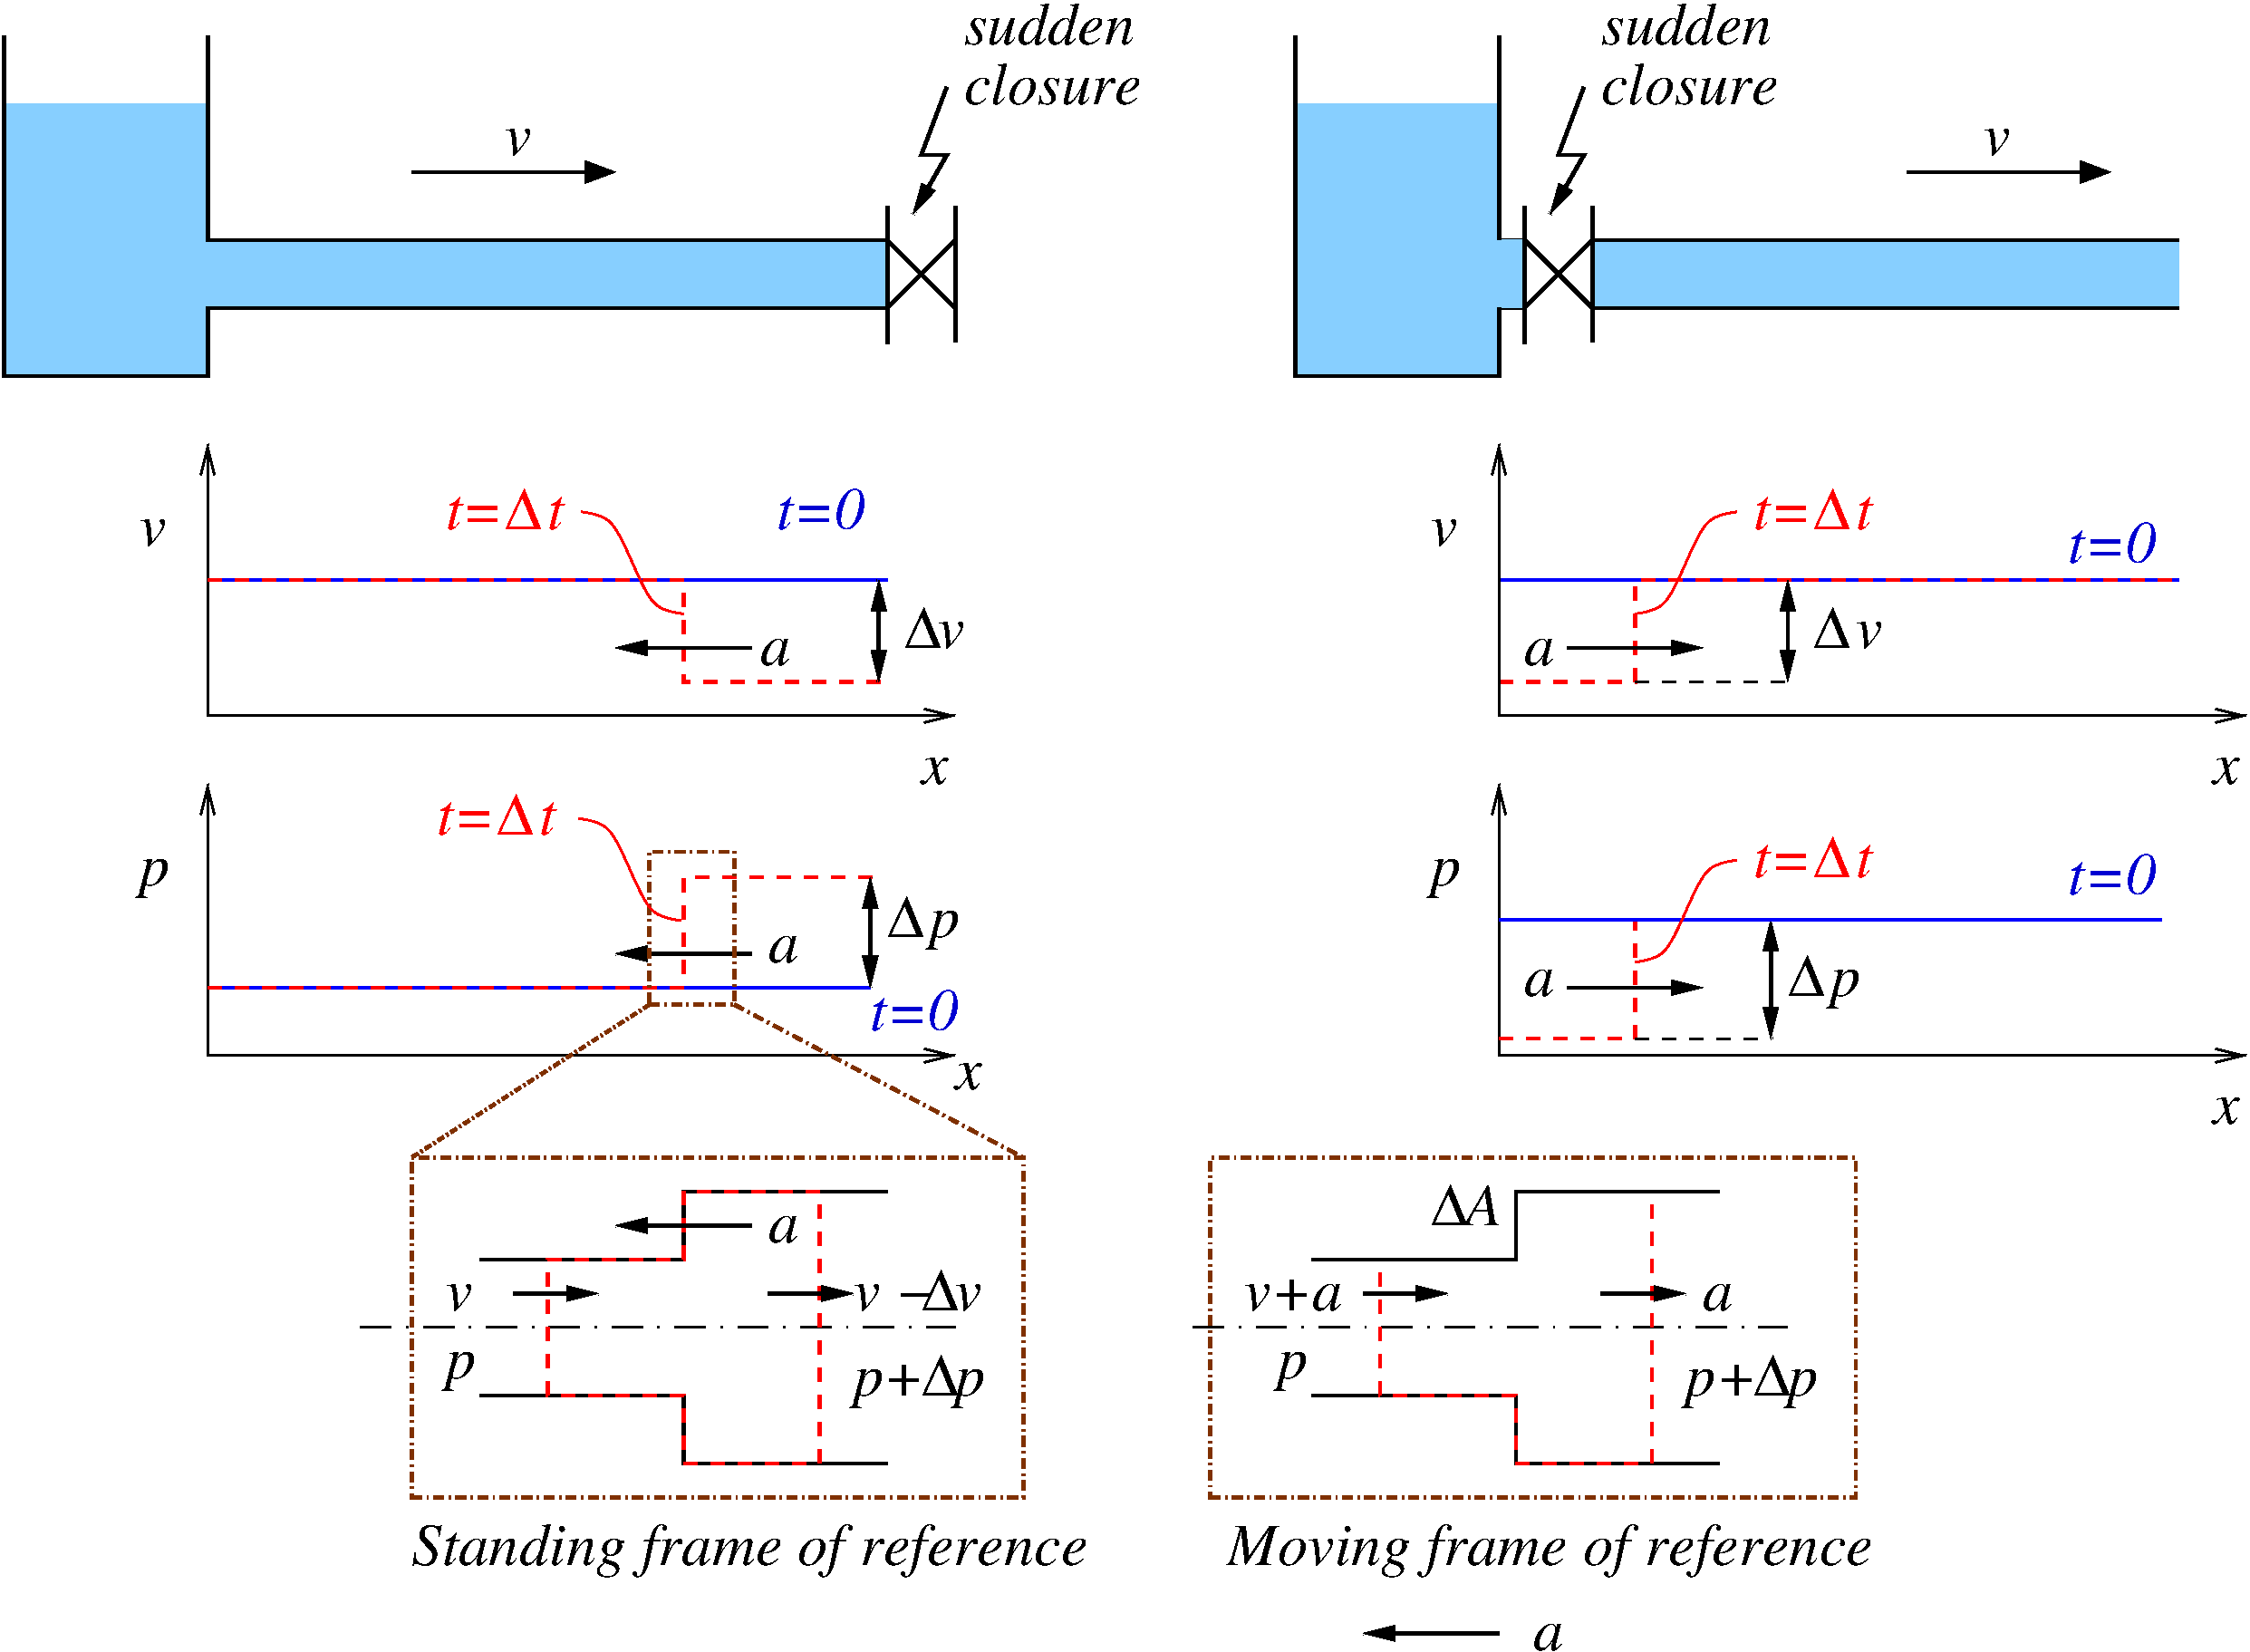
\includegraphics[width=0.8\textwidth]{figs/water_hammer_CV.pdf}
\caption{\label{fig:water_hammer}Water hammer; sudden closure at the (left) end of the pipe and (right) beginning of the pipe.}
%\end{wrapfigure}
\end{figure}

In real situations, the infinitely fast closure of a vale cannot be realised. Instead, a valve is closed by a certain amount of finite time, causing a certain amount of velocity difference ($\Delta v$) in the fluid flow. That is, the liquid is not perfectly stopped; only its velocity is changed. In order to achieve the generated velocity difference, a pressure wave (compression or depression) that provides the energy necessary to decrease the liquid velocity must be built up in the system. The speed of the propagation of the shock front is still $a$. That is, even though the valve is not totally closed, pressure waves with large amplitude can still be presented in the system.

In order to ``feel'' how much energy is contained in a fluid flow in a pipeline, consider a typical configuration of an $L=1\,\mathrm{km}$ long pipe with a diameter of $D=200\,\mathrm{mm}$. Assume that the liquid is water with density $\rho=1000\,\mathrm{kg/m^3}$. The mass of the liquid in the pipe is
%
\begin{equation}
m = \rho L \frac{D^2 \pi}{4} \approx 31.4\,\mathrm{t}.
\end{equation}
%
In order to change the velocity of this mass of water by $\Delta v=1\,\mathrm{m/s}$ within $t=1\,\mathrm{s}$, the required amount of power is
%
\begin{equation}
P = \frac{E_{kin}}{t} = \frac{1}{t} \frac{1}{2} m \Delta v^2 \approx 15.7\,\mathrm{kW},
\end{equation}
%
where $E_{kin}$ is the kinetic energy difference of the liquid.

With the above-described introduction, a quick overview of the phenomenon could be provided. In the rest of the section, we shall proceed with specific calculations and try to answer the following questions. How can the speed of sound $a$ in a pipe or of a pure liquid be calculated? What is the magnitude $\Delta p$ of the generated pressure wave? Furthermore, how it is related to the speed of sound $a$ and the velocity difference $\Delta v$? Finally, how can we avoid/soften the generation of such a pressure wave?

%------------------------------------------------
\subsection{The sound speed in liquids and in pipes}
The propagation of sound (or signal) in any medium is inherently related to the compressibility. In case of an absolutely rigid material (naturally, this assumption is always hypothetical), the sound speed is infinite. That is, any disturbance at a point appears immediately at another point of the material. This is the case for incompressible liquids. Although in many cases, the assumption of incompressibility is a reasonable simplification, in reality, every material is compressible; therefore, a finite speed of sound exists. From thermodynamics, it is well-known that the speed of sound can be calculated from the constitutive law (equation of state) of a substance. For water, the simplest equation of state can be written as
%
\begin{equation} \label{WaterEquationOfState}
p = p_0 + E_f \frac{\rho - \rho_0}{\rho_0},
\end{equation}
%
where $p$ is the pressure, $E_f$ is the bulk (elasticity) modulus of the fluid, and $\rho$ is the density. The subscript $0$ indicates a reference point where both the pressure $p_0$ and the density $\rho_0$ are known. Equation\,\eqref{WaterEquationOfState} expresses a linear relationship between the pressure $p$ and density $\rho$. Observe that the density is increasing with increasing pressure. The second power of the speed of sound can be obtained from the following partial derivative:
%
\begin{equation}
a^2 = \frac{\partial p}{\partial \rho} \approx \frac{\Delta p}{\Delta \rho}
\end{equation}
%
expressing how much pressure difference is necessary to change the density by a single unit. Performing the partial derivative on Eq.\,\ref{WaterEquationOfState}, the speed of sound reads as
%
\begin{equation}
a = \sqrt{ \frac{E_f}{\rho_0} } \approx \sqrt{ \frac{E_f}{\rho} }.
\end{equation}
%
If the density does not change much during the compression/depression, $\rho_0$ can be replaced by a simple mean value of the density denoted by $\rho$. For water, the value of the bulk modulus is approximately $E_f=2.1\,\mathrm{GPa}$, the density is approximately $\rho=1000\,\mathrm{kg/m^3}$; thus, the speed of sound for pure water is about $a=1449\,\mathrm{m/s}$.
 
The above-derived value for sound propagation is valid only for rigid pipes when the elasticity modulus of the pipe is much higher than that of water. If this is not the case, the speed of sound is significantly altered. Due to the elevated (decreased) pressure, the diameter of the pipe is increased (decreased) via elastic deformation. The change in the volume of the pipe acts as if the fluid became more compressible. Note that due to the change of the cross-section, more fluid can be pushed into the pipe. In order to take into account the elasticity of the pipe, a reduced elastic modulus $E_r$ is written as
%
\begin{equation}
\frac{1}{E_r} = \frac{1}{E_f} + \frac{D}{\delta E_p},
\end{equation}
%
where $D$, $\delta$ and $E_p$ are the diameter, thickness and the elastic modulus of the pipe, respectively. Typical values for $E_p$ are ranging between $600\,\mathrm{MPs}$ and $900\,\mathrm{MPa}$. The reduced speed of sound is now defined as
%
\begin{equation}
a = \sqrt{ \frac{E_r}{\rho} }.
\end{equation}
%
Consider a pipe with a diamater of $D=110\,\mathrm{mm}$ and a thickness of $\delta=18.3\,\mathrm{mm}$ with $E_p=800\,\mathrm{MPa}$, the speed of sound is reduced to $a=354\,\mathrm{m/s}$.

%------------------------------------------------
\subsection{Allievi principle: the pressure amplitde for fast closure} \label{sec:pressure_amplitude_fast_closure}

In order to develop sizing equations to avoid water hammer problems, the relationship between the amplitude of the generated pressure wave $\Delta p$ and the velocity change $\Delta v$ need to be found. For this, the macroscopic balances of mass and momentum around the shock front are formulated; and with reasonable simplifications, the required expression shall be established. Consider a frame of reference (co-ordinate system) moving along the pipe together with the shock front with speed $a$. For a better visibility, the related picture in the bottom of Fig.\,\ref{fig:water_hammer} is magnified in Fig.\,\ref{fig:allievi_principle}; thus, additional notations can be added without overcrowding the figure. The vertical dashed line denotes the shock front itself. On the left-hand side of the shock, the pressure and density are $p$ and $\rho$, respectively. The cross-section of the pipe is $A_1$, where the vector $dA_1$ denote the surface element vector. The velocity at this pipe section is $v+a$. The addition of $a$ is necessary as our co-ordinate system is moving with a speed of $a$. Therefore, the two velocities must be added together. On the right-hand side of the shock, the pressure and the density are elevated by $\Delta p$ and $\Delta \rho$, respectively. Moreover, the velocity of the fluid flow is reduced by $\Delta v$. The resulted outflow velocity from the investigated pipe section is $v-\Delta v + a$. Observe that due to the moving reference frame, the addition $a$ is again necessary. The cross-section in the right-hand side is $A_2$ and the corresponding surface element vector is $dA_2$. Due to the increased pressure after the shock front (righ-hand side), the cross section $A_2$ is larger than that of in the left-hand side $A_1$. The difference is $\Delta A = A_2 - A_1$ located at the shock front as a ring shaped surface. Its surface element vector is marked by $d\Delta A$.

\begin{figure}[h!]
\centering
%\begin{wrapfigure}{r}{0.6\textwidth}
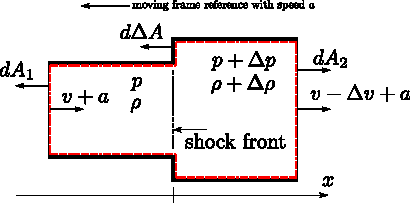
\includegraphics[width=0.6\textwidth]{figs/WaterHammer_AllieviPrinciple.pdf}
\caption{\label{fig:allievi_principle}Shock front in a moving frame reference with speed $a$. The pressure wave is generated by a sudden closure of a valve at the end of the pipe.}
%\end{wrapfigure}
\end{figure}

From elementary fluid dynamics, it is well-know that the macroscopic momentum balance for the fluid package bounded by the red dashed line in Fig.\,\ref{fig:allievi_principle} in an integral form reads as
%
\begin{equation} \label{macroscopic_momentum_balance}
\frac{\partial}{\partial t} \int_V \left(\rho \underline{v} \right) dV + \int_A \rho \underline{v} \left( \underline{v} \cdot d\underline{A} \right) + \int_A p d\underline{A} = \int_V \rho \underline{g} dV.
\end{equation}
%
This integral equation express that the momentum of the bounded fluid package can be changed by forces acting on the bounding surfaces (e.g., pressure, inertia) and on the volume (e.g., gravity). In this equation, $\underline{v}$ denote the velocity vector at a given point on the surface or in the volume in general. In the moving frame co-ordinate system, the fluid flow is stationary; thus, the first integral is identically zero. Moreover, let us neglect the effect of gravity; consequently, the last integral in the right-hand side of Eq.\,\eqref{macroscopic_momentum_balance} is zero as well. The simplified equation is
%
\begin{equation} \label{macroscopic_momentum_balance_simplified}
\int_A \rho \underline{v} \left( \underline{v} \cdot d\underline{A} \right) + \int_A p d\underline{A} = 0.
\end{equation}
%
Observe that in the surface integrals, the surface elements $d\underline{A}$ are vectors, and they are pointing in the outward direction (by convention). In general, performing the integrations in Eq.\,\eqref{macroscopic_momentum_balance_simplified} is a cumbersome task. However, assuming that the velocity vectors are constants (using the mean velocity at every point of the cross-sections) and that they are always perpendicular to the cross-sections, the integrations can be done by elementary calculations. That is, they become simple multiplications of the magnitude of the integrands and the area of the surfaces. It must be stressed that the proper sign of the vectors has to be taken into account. Demonstrate this with an example:
%
\begin{equation}
\int_{A_1} \rho \underline{v} \left( \underline{v} \cdot d\underline{A}_1 \right) = - \rho \left( v+a \right)^2 A_1.
\end{equation}
%
The magnitude of general velocity vector $\underline{v}$ is $v+a$ at cross-section $A_1$. Let the positive direction denoted by $x$, see Fig.\,\ref{fig:allievi_principle}. As the surface element vector $d\underline{A}_1$ is pointing to the negative direction, the value of the integral is negative. Keep in mind that the second power of the velocity vector is always positive regardless of its actual direction. Performing all the integrations in Eq.\,\ref{macroscopic_momentum_balance_simplified} in a similar way for the surfaces $A_1$, $A_2$ and $\Delta A$, the following algebraic equation can be formulated
%
\begin{equation}
- \rho (v+a)^2 A_1 + (\rho+\Delta \rho) (v-\Delta v+a)^2 A_2 - p A_1 - (p+\Delta p) \Delta A + (p+\Delta p) A_2 = 0.
\end{equation}
%
Through the surface $\Delta A$, there is no fluid flow. That is why there is only a pressure-related term associated with this surface. Taking into account that $\Delta A = A_2-A_1$ the above equation simplifies to
%
\begin{equation} \label{simplified_algebraic_equation_of_momentum}
- \rho (v+a)^2 A_1 + (\rho+\Delta \rho) (v-\Delta v+a)^2 A_2 + \Delta p A_1 = 0.
\end{equation}
%
With the help of the continuity equation (conservation of mass)
%
\begin{align}
\dot{m}_{in} &= \dot{m}_{out}, \\
\rho (v+a) A_1 &= (\rho+\Delta \rho) (v-\Delta v+a) A_2,
\end{align}
%
Eq.\,\eqref{simplified_algebraic_equation_of_momentum} is transformed into
%
\begin{equation}
- \rho (v+a)^2 A_1 + \rho (v+a) A_1 (v-\Delta v+a) + \Delta p A_1 = 0.
\end{equation}
%
This equation can be further simplified to
%
\begin{equation}
- \rho (v+a) A_1 \Delta v + \Delta p A_1 = 0.
\end{equation}
%
Eliminating $A_1$ and assuming that the sound speed $a$ (orders of hundreds of $m/s$) is much larger than the flow velocity (orders of $m/s$), the well-known formula for the Allievi principle can be formulated:
%
\begin{equation} \label{allievi_principle}
\Delta p \approx \rho a \Delta v.
\end{equation}

The simple equation of Eq.\,\ref{allievi_principle} expresses that a sudden change in the velocity $\Delta v$ (not necessarily a complete stop of the fluid) initiate a pressure wave with an amplitude of $\Delta p$. Let us assume that the sound speed is $a=350\,\mathrm{m/s}$, the density is $\rho=1000\,\mathrm{kg/m^3}$ and the velocity change is $\Delta v=1\,\mathrm{m/s}$. The generated pressure amplitude is approximate $\Delta p=3.5\,\mathrm{bar}$. 

%------------------------------------------------
\subsection{Pressure amplitude for slow closure} \label{sec:pressure_amplitude_slow_closure}
Intuitively, one can ``feel'' that during a prolonged closure of a valve, the amplitude of the compression/depression waves can be softened. However, Eq.\,\eqref{allievi_principle} is independent from time. Therefore, the validity limit of Eq.\,\eqref{allievi_principle} has to be determined. As it is already discussed in details in Sec.\,\ref{sec:introduction_to_transient_phenomenon}, the initiated pressure wave travels along the pipe. At the other end of the pipe, the pressure wave is reflected and travels back to the valve. During the reflection, the compression wave becomes a depression wave or vice verse. It can be fairly assumed that during the time needed to the pressure wave travelling back and forth, the transient is decayed enough, and a new stationary operation is settled down. This means that Eq.\,\eqref{allievi_principle}, which defines the pressure amplitude of transients, is valid only if the closure of the valve is faster than the characteristic time $T_p$ of the pipe (time needed for the pressure wave travelling back and forth). The value of $T_p$ can be easily calculated from the length of the pipe $L$ and the speed of sound $a$:
%
\begin{equation}
T_p = \frac{2 L}{a}.
\end{equation}
%
If the time of the closure $T_c$ of the valve is smaller than $T_p$, transient phenomenon takes place, the Allievi principle is valid, and the pressure amplitude can be calculated from Eq.\,\eqref{allievi_principle}. Otherwise, the liquid mass in the pipe slows down via quasi-steady states and Newton's second law has to be used:
%
\begin{align}
F &= m \frac{dv}{dt}, \\
\Delta p A &= \rho L A \frac{dv}{dt}.
\end{align}
%
Simplifying with the cross-section $A$ of the pipe, the pressure difference yields
%
\begin{equation} \label{newtons_law_of_water_hammer}
\Delta p = \rho L \frac{dv}{dt} \approx \rho L \frac{\Delta v}{\Delta t}.
\end{equation}
%
As an example, let us assume a pipe length of $L=1000\,\mathrm{m}$, and that the speed of sound is $a=1449\,\mathrm{m/s}$ (rigid pipe wall). Thus, the characteristic time of the pipe $T_p=2L/a=1.38\,\mathrm{s}$. Furthermore, assume that the velocity difference is $\Delta v=1\,\mathrm{m/s}$, the density is $\rho=1000\,\mathrm{kg/m^3}$ and the closure time is $T_c=2\,\mathrm{s}>T_p$. Applying Eq.\,\eqref{newtons_law_of_water_hammer}, the generated pressure amplitude is $\Delta p=5\,\mathrm{bar}$.

%------------------------------------------------
\subsection{Dangerous consequences of the pressure waves}
The pressure amplitude computed either by Eq.\,\eqref{allievi_principle} or Eq.\,\eqref{newtons_law_of_water_hammer} must be superimposed to the actual system pressure either in the positive direction (compression wave/shock wave, left-hand side of Fig.\,\ref{fig:water_hammer}) or in the negative direction (depression wave, right-hand side of Fig.\,\ref{fig:water_hammer}). It must be stressed that both transient and quasi-steady cases are dangerous, see the pressure amplitude calculations of typical examples in Sec.\,\ref{sec:pressure_amplitude_fast_closure} and Sec.\,\ref{sec:pressure_amplitude_slow_closure}. Moreover, both the compression and depression waves can also be dangerous. Assume that the system pressure is $5\,\mathrm{bar}$ and the pressure amplitude is $12\,\mathrm{bar}$. If the pressure wave is a compression wave (valve closure at the end of the pipe, see Fig.\,\ref{fig:water_hammer}), the pipe system has to withstand an elevated peak pressure level of $5+12=17\,\mathrm{bar}$, which can easily result in a pipe burst. On the other hand, when the wave is a depression wave (valve closure at the beginning of the pipe), the theoretical minimum pressure would be $5-12=-7\,\mathrm{bar}$. This is not possible as the liquid/water will evaporate (cavitate), and some sections of the pipe will be filled up with vapour preventing the pressure to drop down below the absolute vacuum. Later on, when the large mass of liquid stops and starts to move back towards the valve (e.g., because the pipe has a slightly positive incline), a large mass of liquid will hit the valve and its surroundings. Also, the pipe can collapse due to the vacuum as shown in the left-hand side of Fig.\,\ref{fig:WaterHammerExamples} (especially with large diameters). Examples for serious damages are shown in Fig.\,\ref{fig:WaterHammerExamples} for depression wave (left-hand side) and compression wave (right-hand side).

\begin{figure}[ht]
\centering
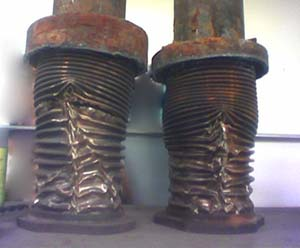
\includegraphics[height=5.5cm]{figs/Water-hammer-blown-expansion-joints.jpg}
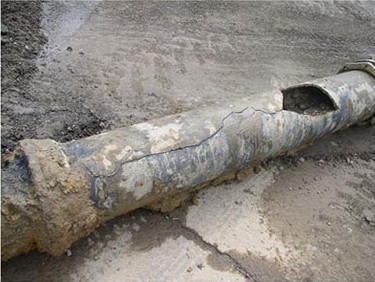
\includegraphics[height=5.5cm]{figs/water_hammer2.jpg}
\caption{\label{fig:WaterHammerExamples} (Left) collapsed expansion joints due to depression wave. (Right) pipe burst due to chock wave (compression wave).}
\end{figure}

%------------------------------------------------
\subsection{Summary and prevention of water hammer}

Before the discussion of techniques to avoid water hammer phenomenon, let us summarize the findings of the previous sections via some bullet points:

\begin{itemize}
\item Closure of valves results in pressure waves $\Delta p$ due to the change of the velocity of the fluid flow. In this sense, any ``action'' causing a velocity difference can also cause pressure waves (e.g., starte and shut down of pumps). Sometimes the phenomenon is related to a complicated interaction of devices; for example, the sudden closure of a check valve (prevent backflow of the liquid) during the shut down of a pump. 
\item The speed $a$ of the propagating pressure wave depends on the equation of state of the liquid and the material properties of the pipe.
\item If the closure time $T_c$ is smaller than the characteristic time of the pipe $T_p$, the pressure amplitude is obtained from the Allievi principle Eq.\,\eqref{allievi_principle}; otherwise, it can be calculated from Newton's second law Eq.\,\eqref{newtons_law_of_water_hammer}.
\item Both the compression and depression waves are dangerous for the system. However, due to the possible cavitation effect and the collapse of the pipe (especially for large diameters), the depression wave is usually more dangerous.
\end{itemize}

As water hammer is an undesirable phenomenon, many techniques have been developed to avoid its harmful consequences. Let us summarize them again via some bullet points:

\begin{itemize}
\item Keep the fluid velocity low. The smaller the possible velocity difference, the smaller the generated pressure amplitude. 
\item Close the valve, shut down or start the pump slowly or in a controlled manner.
\item Use air vessels that are large tanks half-filled with air. The highly compressible gas inside can significantly soften the pressure waves. That is, it acts as a ``shock absorber''. The disadvantage is the high investment costs.
\item Air valves are often used to remediate the consequences of low pressure in a depression wave by releasing air into the pipe. Thus, the pressure inside the pipe cannot be lower than the ambient pressure of the environment. Moreover, the air also cushions the effect when the large mass of liquid starts to move backwards and tries to hit the valve or the pump, see the discussion of the previous section.
\end{itemize}

%------------------------------------------------
\subsection{Problems}


%%%%%%%%%%%%%%%%%%%%%%%%%%%%%%%%%%%%%%%%%%%%%%%%%%%%%%%%%%%%%%%%%%%%

\vspace{1cm}
\noindent {\bf Problem \thesection.\theprob}\stepcounter{prob}

The diameter of a pipe is NA150, the volumetric flow rate us $Q=44~\frac{\mathrm{m^3}}{\mathrm{h}}$, the \emph{relative} pressure in the pipe is $5~\mathrm{bar}$, and the sonic velocity is $a=1200~\frac{\mathrm{m}}{\mathrm{s}}$. Find the amplitude of the pressure wave, in case when the pump at the beginning of the pipe suddenly stops! The flow velocity reaches zero faster than the characteristic time of the pipe, therefore Allievi's theory can be used. Is cavitation possible in the pipe? For the same volumetric flow rate, find the diameter of the pipe, at which cavitation is no longer possible!

Solution:

Allievi's theory states that
\begin{align*}
\Delta p = \rho a \Delta v.
\end{align*}
The velocity of the fluid in then pipe is
\begin{align*}
v = \frac{Q}{A} = \frac{4Q}{D^2 \pi} = \frac{4\cdot 44}{0.15^2 \cdot \pi \cdot 3600} = 0.69~\frac{\mathrm{m}}{\mathrm{s}}.
\end{align*}
The amplitude of the pressure rate is given by
\begin{align*}
\Delta p = 1000 \cdot 1200 \cdot 0.69 = 828 000 ~\mathrm{Pa} = 8.3~\mathrm{bar}.
\end{align*}
Knowing the amplitude of the pressure wave and the relative pressure in the pipe, the smallest relative pressure possible in the pipe is $5-8.3 = -3.3~\mathrm{bar}$. This is impossible, the smallest relative pressure possible is $-1~\mathrm{bar}$. Below 0 bar relative pressure, cavitation is possible. To avoid this, the required pipe diameter is
\begin{align*}
\Delta p = \rho a \Delta v = \rho a \frac{4Q}{D^2 \pi} \rightarrow D = \sqrt{\rho a \frac{4Q}{\Delta p \pi}} = \sqrt{1000 \cdot 1200 \cdot \frac{4\cdot 44}{5 \cdot 10^5 \pi \cdot 3600}} = 0.193~\mathrm{m}
\end{align*}
Therefore, with an NA200 pipe, caviation can be avoided when the pipe is closed faster than the characteristic time of the pipe.


%%%%%%%%%%%%%%%%%%%%%%%%%%%%%%%%%%%%%%%%%%%%%%%%%%%%

\vspace{1cm}
\noindent {\bf Problem \thesection.\theprob}\stepcounter{prob}

During the reconstruction of a water pipe, the old asbestos cement (AC) pipe is changed to a steel pipe. The sonic speed is $a_{AC}=920~\frac{\mathrm{m}}{\mathrm{s}}$ and $a_{steel}=1200~\frac{\mathrm{m}}{\mathrm{s}}$ in the asbestos cement and steel pipe, respectively. The velocity of the fluid is $0.7~\frac{\mathrm{m}}{\mathrm{s}}$, and the pressure is $p=7~\mathrm{bar}$. Find the amplitude of the pressure wave for both pipes, assuming the end of the pipe is closed fast (under the characteristic time)!

(Solution: AC: $dp=6.44~\mathrm{bar}$, $p_{max} = 13.44~\mathrm{bar}$. Steel pipe: $dp=8.4~\mathrm{bar}$, $p_{max} = 15.4~\mathrm{bar}$)

%%%%%%%%%%%%%%%%%%%%%%%%%%%%%%%%%%%%%%%%%%%%%%%%%%%%

\vspace{1cm}
\noindent {\bf Problem \thesection.\theprob}\stepcounter{prob}

A NA200 pipe that's length is $8~\mathrm{km}$, conveys water to an open reservoir. The volumetric flow rate is $Q=3600~\frac{\mathrm{l}}{\mathrm{min}}$, and the end of the pipe is above the water level of the reservoir. The friction factor is $\lambda=0.018$. Find the pressure at the beginning of the pipe! Assuming that the velocity decreases linearly in time, find the ratio of the characteristic time of the pipe and the time under which the valve at the pressure side of the pump can be closed! The criteria is that the pressure cannot be lower than the atmospheric pressure! The sonic speed is $a=1200~\frac{\mathrm{m}}{\mathrm{s}}$. Find the characteristic time of the pipe! Plot the velocity of the fluid as a function of time!

(Solution: $p=13.13~\mathrm{bar}$, $\frac{T}{T_{char}} = 1.75$, $T_{char} = 13.33~\mathrm{s}$)


\clearpage